% Options for packages loaded elsewhere
\PassOptionsToPackage{unicode}{hyperref}
\PassOptionsToPackage{hyphens}{url}
\documentclass[
  preprint,12pt]{elsarticle}
\usepackage{xcolor}
\usepackage[margin=1in]{geometry}
\usepackage{amsmath,amssymb}
\setcounter{secnumdepth}{5}
\usepackage{iftex}
\ifPDFTeX
  \usepackage[T1]{fontenc}
  \usepackage[utf8]{inputenc}
  \usepackage{textcomp} % provide euro and other symbols
\else % if luatex or xetex
  \usepackage{unicode-math} % this also loads fontspec
  \defaultfontfeatures{Scale=MatchLowercase}
  \defaultfontfeatures[\rmfamily]{Ligatures=TeX,Scale=1}
\fi
\usepackage{lmodern}
\ifPDFTeX\else
  % xetex/luatex font selection
  \setmainfont[]{Times New Roman}
  \setmathfont[]{STIX Two Math}
\fi
% Use upquote if available, for straight quotes in verbatim environments
\IfFileExists{upquote.sty}{\usepackage{upquote}}{}
\IfFileExists{microtype.sty}{% use microtype if available
  \usepackage[]{microtype}
  \UseMicrotypeSet[protrusion]{basicmath} % disable protrusion for tt fonts
}{}
\makeatletter
\@ifundefined{KOMAClassName}{% if non-KOMA class
  \IfFileExists{parskip.sty}{%
    \usepackage{parskip}
  }{% else
    \setlength{\parindent}{0pt}
    \setlength{\parskip}{6pt plus 2pt minus 1pt}}
}{% if KOMA class
  \KOMAoptions{parskip=half}}
\makeatother
\usepackage{longtable,booktabs,array}
\newcounter{none} % for unnumbered tables
\usepackage{calc} % for calculating minipage widths
% Correct order of tables after \paragraph or \subparagraph
\usepackage{etoolbox}
\makeatletter
\patchcmd\longtable{\par}{\if@noskipsec\mbox{}\fi\par}{}{}
\makeatother
% Allow footnotes in longtable head/foot
\IfFileExists{footnotehyper.sty}{\usepackage{footnotehyper}}{\usepackage{footnote}}
\makesavenoteenv{longtable}
\usepackage{graphicx}
\makeatletter
\newsavebox\pandoc@box
\newcommand*\pandocbounded[1]{% scales image to fit in text height/width
  \sbox\pandoc@box{#1}%
  \Gscale@div\@tempa{\textheight}{\dimexpr\ht\pandoc@box+\dp\pandoc@box\relax}%
  \Gscale@div\@tempb{\linewidth}{\wd\pandoc@box}%
  \ifdim\@tempb\p@<\@tempa\p@\let\@tempa\@tempb\fi% select the smaller of both
  \ifdim\@tempa\p@<\p@\scalebox{\@tempa}{\usebox\pandoc@box}%
  \else\usebox{\pandoc@box}%
  \fi%
}
% Set default figure placement to htbp
\def\fps@figure{htbp}
\makeatother
\setlength{\emergencystretch}{3em} % prevent overfull lines
\providecommand{\tightlist}{%
  \setlength{\itemsep}{0pt}\setlength{\parskip}{0pt}}
\usepackage{graphicx}
\usepackage{bookmark}
\IfFileExists{xurl.sty}{\usepackage{xurl}}{} % add URL line breaks if available
\urlstyle{same}
\hypersetup{
  pdftitle={VoltGuard: Topology-Aware Voltage-Risk Screening with Conformal Calibration for Active Distribution Networks},
  pdfauthor={Siqiang Zhao (corresponding author), Fengxiang Zhang},
  hidelinks,
  pdfcreator={LaTeX via pandoc}}

\title{VoltGuard: Topology-Aware Voltage-Risk Screening with Conformal
Calibration for Active Distribution Networks}
\author{Siqiang Zhao (corresponding author), Fengxiang Zhang}
\date{Generated 2026-07-03 02:10 UTC}

\begin{document}
\maketitle

\section*{Title Page}\label{title-page}
\addcontentsline{toc}{section}{Title Page}

\textbf{Journal:} Energy Conversion and Management: X

\textbf{Article title:} VoltGuard: Topology-Aware Voltage-Risk Screening
with Conformal Calibration for Active Distribution Networks

\textbf{Authors and affiliations:}

Siqiang Zhao\(^{a,*}\); Fengxiang Zhang\(^{b}\)

\(^{a}\) Sichuan University-Pittsburgh Institute, Chengdu, China

\(^{b}\) Southwest Jiaotong University, Chengdu, China

\(^{*}\) Corresponding author. Email: 2023141520257@stu.scu.edu.cn

\section*{Abstract}\label{abstract}
\addcontentsline{toc}{section}{Abstract}

High photovoltaic penetration, electric-vehicle charging, and flexible
demand make voltage-risk screening in active distribution networks
increasingly uncertain. VoltGuard provides a calibrated screening layer
that combines a squared-voltage LinDistFlow physical backbone,
topology-aware residual learning, and topology/PV/loading conditioned
split conformal calibration. The method converts pre-dispatch operating
forecasts into voltage-risk intervals that are sharp enough for scenario
triage while maintaining high recall of voltage-limit crossings.
Experiments on IEEE 33-bus and IEEE 69-bus distribution feeders, with an
expanded IEEE 118-bus stress audit, show that topology/PV/loading
conditioned calibration improves the coverage-sharpness-risk tradeoff
relative to global conformal calibration, tree-based point screens, and
a neural graph residual ablation. On the representative 33/69 random
split, VoltGuard achieves 0.00011 p.u. RMSE, 93.66\% empirical coverage
for nominal 90\% intervals, 99.89\% bus-level violation recall, and one
missed bus-level violation. Across three random seeds, the method
reduces mean missed violations from 1.67 to 0.33 while cutting mean
interval width from 0.00127 to 0.00049 p.u. Runtime measurements show
0.254 ms/scenario online screening versus 1725 ms/scenario for the
AC-audited grid-search backend, making VoltGuard a practical front end
for prioritizing downstream AC analysis.

\section*{Keywords}\label{keywords}
\addcontentsline{toc}{section}{Keywords}

Physics-informed machine learning; Conformal prediction; Topology-aware
learning; Active distribution networks; Voltage security; Risk
screening; Renewable hosting

\section{Introduction}\label{introduction}

Active distribution networks are increasingly operated close to voltage
limits while being asked to host more renewable generation. Rooftop PV,
electric-vehicle charging, flexible loads, storage, and feeder switching
create operating points that vary faster than classical planning margins
were designed to handle. Voltage violations are costly in both
directions: undervoltage degrades service quality and equipment
operation, whereas overvoltage can force renewable curtailment or
protection actions. The resulting problem is not only a
voltage-estimation problem: operators need calibrated uncertainty around
voltage-risk estimates before deciding which scenarios deserve
downstream AC analysis.

Machine-learning voltage predictors are attractive because they can
rapidly map forecasts and pseudo-measurements to voltage estimates.
However, point accuracy is not enough for operation. A predictor with
low RMSE can still miss rare voltage-limit crossings, and a globally
conservative interval can produce so many false alarms that the operator
no longer trusts it. The useful operational object is therefore a
calibrated voltage-risk interval: an interval that is sharp enough to
screen many safe scenarios, yet conservative enough to reduce missed
violations near the 0.95-1.05 p.u. operating band.

This paper frames the task as calibrated voltage-risk screening. The
proposed method, VoltGuard, uses a LinDistFlow physical backbone to
encode feeder structure, learns a topology-aware residual correction
from available operating features, and then uses split conformal
calibration to convert residual errors into voltage intervals. The
contribution is positive and operational: a fast, auditable screen that
ranks scenarios and buses before AC analysis is invoked.

The contribution is intentionally not ``a stronger GNN.'' A lightweight
neural graph residual is included as an ablation, but the selected
estimator is the topology-aware residual learner with conditioned
conformal calibration because it gives the best risk-sharpness tradeoff
in the executed experiments.

The paper makes three contributions:

\begin{enumerate}
\def\labelenumi{\arabic{enumi}.}
\tightlist
\item
  A reproducible physics-informed topology-aware residual model that
  corrects a squared-voltage LinDistFlow backbone using only operating
  information available before AC labels are observed.
\item
  A topology/PV/loading conditioned split conformal calibration
  procedure with shrinkage fallback for voltage-risk intervals.
\item
  A focused screening evaluation on IEEE 33-bus and IEEE 69-bus
  distribution feeders showing how calibrated intervals affect coverage,
  interval width, false alarms, and missed-voltage-risk behavior.
\end{enumerate}

The remaining audits, including EV-conditioning sensitivity,
calibration-budget checks, candidate-action pruning, and high-PV hosting
stress, are supporting application extensions. They are not used to
define the central method claim.

\subsection{Scope and Companion-Paper
Positioning}\label{scope-and-companion-paper-positioning}

This manuscript is the core screening-method paper. A companion DMS
integration paper specifies deployment contracts, queue semantics,
fallback rules, and operator audit records for using calibrated
voltage-risk screens in control centers. A separate
LinDistFlow-global-quantile note defines a minimal reference baseline.
The three papers are parallel companion studies: this paper answers how
to estimate calibrated voltage-risk intervals, the DMS paper answers how
such intervals should be embedded in operations, and the baseline note
answers what a transparent physical proxy plus one pooled quantile can
achieve.

VoltGuard gives calibrated voltage-risk intervals under a stated
feeder/scenario/split/calibration protocol. It complements AC power
flow, OPF, and MPC by deciding which scenarios deserve immediate
downstream analysis. AC feasibility, final dispatch, protection action,
and closed-loop control remain the responsibility of those downstream
tools.

\begin{figure}
\centering
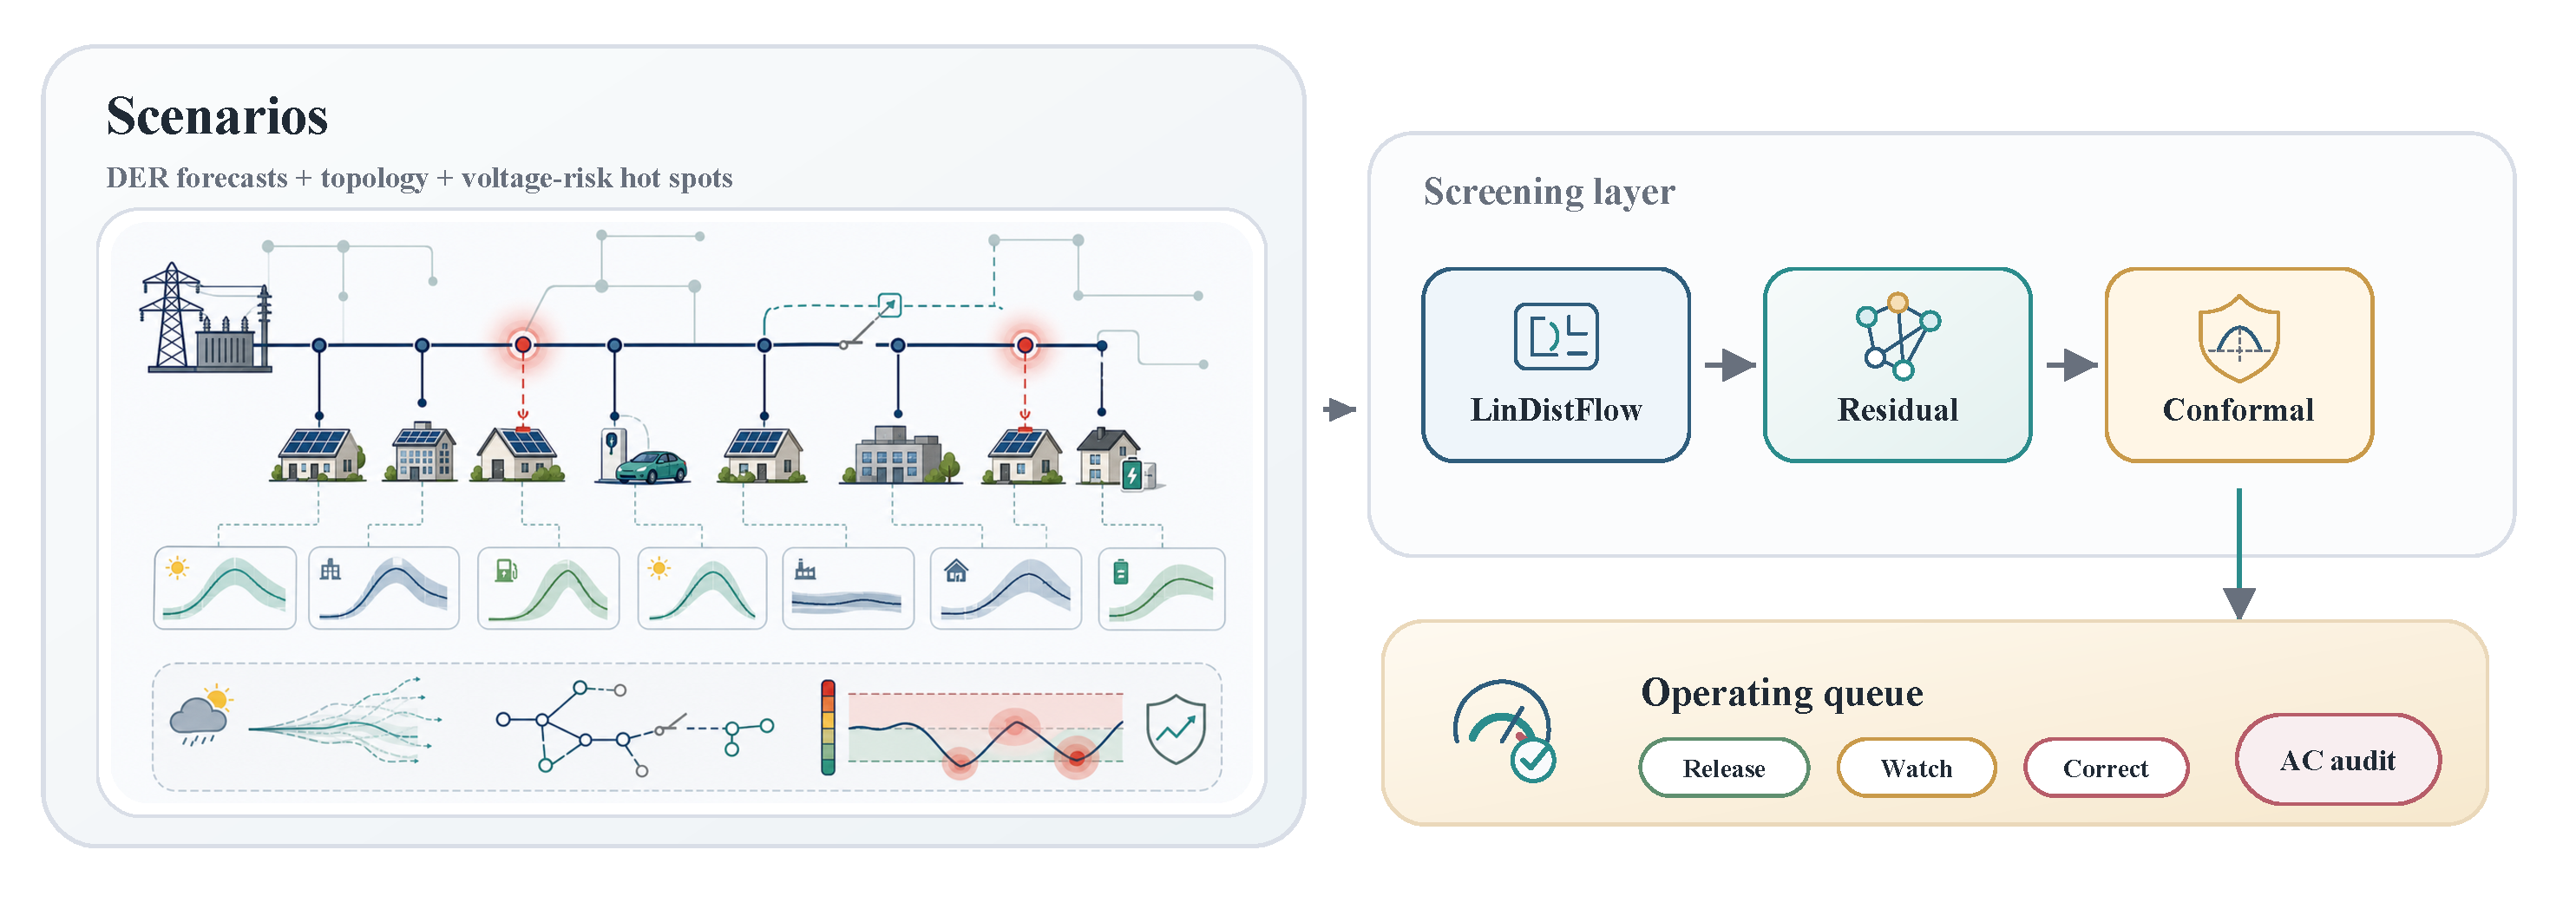
\includegraphics[width=1.1\linewidth,height=\textheight,keepaspectratio,alt={Graphical abstract and VoltGuard screening workflow. The figure summarizes the active-feeder inputs, LinDistFlow physical backbone, topology-aware residual correction, conformal voltage-risk intervals, and downstream AC-audited corrective optimization interface.}]{figures/fig01_graphical_abstract_workflow.pdf}
\caption{Graphical abstract and VoltGuard screening workflow. The figure
summarizes the active-feeder inputs, LinDistFlow physical backbone,
topology-aware residual correction, conformal voltage-risk intervals,
and downstream AC-audited corrective optimization
interface.}\label{fig:fig01_graphical_abstract_workflow}
\end{figure}

\section{Related Work}\label{related-work}

Classical distribution-voltage assessment uses AC power flow,
distribution state estimation, optimal power flow, Volt-VAR control, and
conservative operating margins. Distribution feeder reconfiguration and
DistFlow-style approximations trace back to radial-feeder power-flow
models used for loss reduction and load balancing {[}1{]}. LinDistFlow
and related approximations are valuable because they expose how
downstream active and reactive power flows drive voltage drops. Their
accuracy degrades under losses, reverse power flow, unmodeled imbalance,
and uncertain injections, but they remain useful physical backbones for
fast screening. OPF and distributed control remain the stronger
corrective layers when an operating point requires actual dispatch
decisions {[}2,3{]}.

Physics-informed learning for power systems embeds network equations,
line parameters, topology, or power-flow residuals into data-driven
predictors. This improves interpretability and can reduce the burden on
a black-box model. Recent physics-informed graph learning work for
power-system state estimation also illustrates the value of combining
electrical structure with learnable corrections {[}4{]}. In this work,
the residual target is deliberately smaller than direct voltage
prediction: the learner corrects a physical voltage proxy rather than
replacing feeder physics.

Graph neural networks are natural for power grids because buses and
lines form a graph. General graph-convolution and inductive
representation-learning methods provide the modeling background for
message passing on networks {[}5,6{]}. Many grid-learning studies
emphasize point prediction, state estimation, or OPF acceleration. This
paper treats graph-neural modeling as relevant background but not as the
main claim. The executed neural graph residual is retained as an
ablation and is not used to justify the title or contribution.

Conformal prediction converts arbitrary predictors into calibrated
prediction sets or intervals under exchangeability assumptions
{[}7,8{]}. Conformalized quantile regression further shows why interval
efficiency matters, not only nominal coverage {[}9{]}. Recent
conformalized GNN work highlights two difficulties that matter here:
graph-structured samples may not be exchangeable in the usual i.i.d.
sense, and intervals can become too wide if calibration ignores topology
or operating regime {[}10,11{]}. VoltGuard addresses this operationally
by conditioning calibration on feeder, PV, and loading families, then
reporting per-family coverage and interval width rather than hiding all
calibration behavior in a single global number.

Table 1 positions the paper relative to representative technical lines.
The comparison is not a claim that every cited method solves the same
screening task; it identifies the missing combination that motivates
VoltGuard.

{\def\LTcaptype{none} % do not increment counter
\begin{longtable}[]{@{}
  >{\raggedright\arraybackslash}p{(\linewidth - 8\tabcolsep) * \real{0.1579}}
  >{\raggedleft\arraybackslash}p{(\linewidth - 8\tabcolsep) * \real{0.2105}}
  >{\raggedleft\arraybackslash}p{(\linewidth - 8\tabcolsep) * \real{0.2105}}
  >{\raggedleft\arraybackslash}p{(\linewidth - 8\tabcolsep) * \real{0.2105}}
  >{\raggedleft\arraybackslash}p{(\linewidth - 8\tabcolsep) * \real{0.2105}}@{}}
\toprule\noalign{}
\begin{minipage}[b]{\linewidth}\raggedright
Line of work
\end{minipage} & \begin{minipage}[b]{\linewidth}\raggedleft
Physics model
\end{minipage} & \begin{minipage}[b]{\linewidth}\raggedleft
Topology-aware learning
\end{minipage} & \begin{minipage}[b]{\linewidth}\raggedleft
Calibrated interval
\end{minipage} & \begin{minipage}[b]{\linewidth}\raggedleft
Screening/DMS interface
\end{minipage} \\
\midrule\noalign{}
\endhead
\bottomrule\noalign{}
\endlastfoot
AC OPF and distribution control {[}2,3,14-16{]} & yes & model based & no
& corrective backend \\
Learning-assisted OPF/control {[}17,18,20{]} & partial & sometimes &
usually no & dispatch-oriented \\
Physics-aware state estimation {[}4,19{]} & yes & yes & usually no &
estimation-oriented \\
Conformal prediction and CQR {[}7-9,22-24{]} & model agnostic & no & yes
& task agnostic \\
Conformalized GNNs {[}10,11{]} & no explicit feeder physics & yes & yes
& graph prediction \\
VoltGuard & LinDistFlow backbone & yes & topology/PV/loading conditioned
& voltage-risk screening \\
\end{longtable}
}

\section{Problem Formulation}\label{problem-formulation}

Consider a distribution feeder

\[
\mathcal{G}=(\mathcal{N},\mathcal{E}),
\]

where \(\mathcal{N}\) is the bus set and \(\mathcal{E}\) is the branch
set. A root or slack bus \(0\) defines branch orientation: each branch
\((i,j)\in\mathcal{E}\) is directed from upstream bus \(i\) toward
downstream bus \(j\). Each branch has resistance \(r_{ij}\) and
reactance \(x_{ij}\). Let \(v_{i,t}\) be voltage magnitude at bus \(i\)
in scenario \(t\), and let

\[
u_{i,t}=v_{i,t}^2
\]

be squared voltage magnitude. The slack voltage is fixed to
\(v_{0,t}=1.0\) p.u. in the executed simulations, hence \(u_{0,t}=1.0\).

The operating features available before screening are load forecasts or
pseudo-measurements \(p^d_{i,t}, q^d_{i,t}\), PV forecasts
\(p^g_{i,t}\), EV-load indicators, feeder topology, and local/neighbor
electrical features. Net injection is written as

\[
p_{i,t}=p^d_{i,t}-p^g_{i,t}, \qquad q_{i,t}=q^d_{i,t}-q^g_{i,t}.
\]

Positive \(p_{i,t}\) denotes net demand. AC power-flow labels
\(v^\star_{i,t}\) are used only for supervised training, calibration
scoring, and test evaluation. Test labels are never used to construct
features or conformal radii.

The goal is to produce calibrated voltage intervals

\[
\widehat{\mathcal{I}}^{1-\alpha}_{i,t}
= [\hat v^L_{i,t},\hat v^U_{i,t}]
\]

that are sharp enough for operation while limiting missed voltage
violations. The bus-level risk flag is

\[
\rho_{i,t} =
\mathbf{1}\{\hat v^L_{i,t}<v^{\min}\ \mathrm{or}\ \hat v^U_{i,t}>v^{\max}\},
\]

with \(v^{\min}=0.95\) p.u. and \(v^{\max}=1.05\) p.u. The
scenario-level flag is

\[
\rho_t^{\max} = \max_{i\in\mathcal{N}}\rho_{i,t}.
\]

For prioritization, VoltGuard also computes a scenario-level interval
risk score

\[
\eta_t =
\max_{i\in\mathcal{N}}
\left[
\max(0,v^{\min}-\hat v^L_{i,t}),
\max(0,\hat v^U_{i,t}-v^{\max})
\right].
\]

Large \(\eta_t\) means that at least one calibrated bus interval crosses
a voltage limit by a larger margin, so the scenario should be considered
earlier by downstream AC-audited corrective optimization.

\section{Methodology}\label{methodology}

\subsection{LinDistFlow Backbone}\label{lindistflow-backbone}

For each scenario, approximate downstream branch flows are computed from
the forecast net injections and the oriented radial feeder tree:

\[
\hat P_{ij,t} = \sum_{k\in\mathcal{D}(j)} p_{k,t}, \qquad
\hat Q_{ij,t} = \sum_{k\in\mathcal{D}(j)} q_{k,t},
\]

where \(\mathcal{D}(j)\) is the downstream subtree rooted at bus \(j\).
The squared-voltage LinDistFlow recursion is

\[
\hat u^{lin}_{j,t} =
\hat u^{lin}_{i,t} - 2(r_{ij}\hat P_{ij,t}+x_{ij}\hat Q_{ij,t}),
\qquad \hat u^{lin}_{0,t}=1.
\]

The voltage-magnitude proxy is

\[
\hat v^{lin}_{i,t}=\sqrt{\max(\hat u^{lin}_{i,t},\epsilon)},
\]

where \(\epsilon>0\) prevents numerical issues. The executable prototype
computes this squared-voltage backbone explicitly and stores both
\(\hat u^{lin}_{i,t}\) and \(\hat v^{lin}_{i,t}\). These quantities are
used as residual targets and model inputs together with bus position,
voltage base, degree, load, PV, net demand, neighbor load/PV/net demand,
load scale, PV penetration, and EV scale. No test AC voltage label is
used to build the LinDistFlow proxy, conformal radius, or test-time risk
flag.

\subsection{Topology-Aware Residual
Learner}\label{topology-aware-residual-learner}

VoltGuard predicts a voltage-magnitude residual

\[
\Delta \hat v_{i,t}=f_\theta(x_{i,t},z_{i,t},g_i),
\]

where \(x_{i,t}\) contains local bus operating features, \(z_{i,t}\)
contains neighbor-aggregated electrical features, and \(g_i\) contains
topology features such as normalized bus index, slack indicator, voltage
base, and degree. The final point estimate is

\[
\hat v_{i,t} = \hat v^{lin}_{i,t} + \Delta \hat v_{i,t}.
\]

In the executable implementation, \(f_\theta\) is an ExtraTrees residual
learner trained on \(v^\star_{i,t}-\hat v^{lin}_{i,t}\). This choice is
deliberate: it is stable on the executed feeder/scenario families and
outperforms the lightweight neural graph residual on the point-error,
interval-width, and false-alarm metrics used for the selected model.

\subsection{Physics-Informed
Objective}\label{physics-informed-objective}

The supervised residual objective is

\[
\mathcal{L}_{sup}
= \frac{1}{|\mathcal{T}||\mathcal{N}|}
\sum_{t\in\mathcal{T}}\sum_{i\in\mathcal{N}}
\left(\hat v_{i,t}-v^\star_{i,t}\right)^2 .
\]

The physics residual used to define the reproducible model class is a
branch-level voltage-drop mismatch in squared-voltage space:

\[
\mathcal{R}_{drop}
= \frac{1}{|\mathcal{T}||\mathcal{E}|}
\sum_{t\in\mathcal{T}}\sum_{(i,j)\in\mathcal{E}}
\left(
\hat u_{j,t}-\hat u_{i,t}
+2(r_{ij}\hat P_{ij,t}+x_{ij}\hat Q_{ij,t})
\right)^2 .
\]

Here \(\hat u_{i,t}=\hat v_{i,t}^2\) after residual correction, and
\(\hat P,\hat Q\) are computed from forecast injections and feeder
orientation, not from test labels. A smoothness penalty may be added as

\[
\mathcal{R}_{smooth}
= \frac{1}{|\mathcal{T}||\mathcal{E}|}
\sum_{t,(i,j)}
\frac{(\hat v_{i,t}-\hat v_{j,t})^2}{r_{ij}^2+x_{ij}^2+\epsilon}.
\]

The full conceptual objective is

\[
\mathcal{L}
= \mathcal{L}_{sup}
+\lambda_{drop}\mathcal{R}_{drop}
+\lambda_{smooth}\mathcal{R}_{smooth}.
\]

The current tree-based residual implementation realizes the same
philosophy through physics-derived inputs and residual targets rather
than through gradient-based neural optimization of all penalty terms.
The physics residual is still reported explicitly so that a neural or
differentiable implementation can reproduce the same objective without
changing the paper's model boundary.

\subsection{Split Conformal
Calibration}\label{split-conformal-calibration}

For a calibration set \(\mathcal{C}\) disjoint from training and
testing, the nonconformity score is

\[
s_{i,t}=|v^\star_{i,t}-\hat v_{i,t}|.
\]

For nominal miscoverage \(\alpha\), global split conformal calibration
uses

\[
\hat q_{1-\alpha}
= \mathrm{Quantile}_{\lceil (|\mathcal{C}|+1)(1-\alpha)\rceil/|\mathcal{C}|}
\{s_{i,t}:(i,t)\in\mathcal{C}\}.
\]

The global interval is

\[
\widehat{\mathcal{I}}^{1-\alpha}_{i,t}
= [\hat v_{i,t}-\hat q_{1-\alpha},
   \hat v_{i,t}+\hat q_{1-\alpha}].
\]

The finite-sample conformal statement relies on exchangeability between
calibration and test samples {[}7,8{]}. In this paper, that means the
stated feeder/scenario family, split rule, and calibration protocol. The
paper does not claim unconditional safety under arbitrary topology
switching, time drift, PV distribution shift, or field deployment.

\subsection{Topology/PV/Loading Conditioned
Calibration}\label{topologypvloading-conditioned-calibration}

Voltage residual distributions vary by feeder, PV level, and loading
regime. VoltGuard therefore partitions calibration samples into families

\[
g(i,t)=\{\mathrm{feeder},\mathrm{PV\ bin},\mathrm{load\ bin}\}.
\]

For each family \(g\), a family quantile \(\hat q_{g,1-\alpha}\) is
computed. To avoid overconfident intervals in small families, VoltGuard
uses shrinkage toward the global quantile:

\[
\tilde q_{g,1-\alpha}
= \omega_g\hat q_{g,1-\alpha}
+(1-\omega_g)\hat q_{1-\alpha},
\qquad
\omega_g=\frac{n_g}{n_g+n_0},
\]

where \(n_g\) is the number of calibration samples in family \(g\) and
\(n_0\) is the minimum-group scale. The experiments compare global,
PV-conditioned, topology-conditioned, topology+PV+loading conditioned,
and no-shrinkage variants. EV scale is included in the point-estimator
feature set, but it is not automatically used as a conformal grouping
key because it can fragment family sample sizes. The EV-conditioned
ablation in the results tests this choice directly.

\subsection{Two-Stage Operating
Interface}\label{two-stage-operating-interface}

VoltGuard is a screening layer. It does not select final dispatch as an
OPF or MPC controller. In the two-stage interface:

\begin{enumerate}
\def\labelenumi{\arabic{enumi}.}
\tightlist
\item
  VoltGuard produces calibrated bus-level intervals and scenario-level
  risk flags.
\item
  Risky scenarios are passed to an AC-audited corrective layer, such as
  discrete grid search, OPF, or MPC.
\item
  When the downstream layer has limited compute budget, scenarios are
  ranked by \(\eta_t\) so that larger interval-limit crossings are
  audited first.
\end{enumerate}

The simple risk-trigger action used for diagnostic operating value
applies 10\% flexible-load relief when undervoltage risk appears and
10\% PV curtailment when overvoltage risk appears. A stronger AC-audited
grid search is then reported as a downstream corrective benchmark.

\section{Experimental Design}\label{experimental-design}

The main experiments use IEEE 33-bus and IEEE 69-bus distribution
feeders. IEEE 118-bus is retained as a supplementary stress test because
it is not a canonical distribution feeder. For each feeder, 300
AC-solvable scenarios are generated with randomized load scale, PV
penetration, EV demand, and PV siting. AC power flow provides reference
labels.

Four split protocols are executed:

\begin{itemize}
\tightlist
\item
  Random interpolation: scenario-disjoint 60/20/20
  train/calibration/test split.
\item
  Synthetic time-block: scenario IDs are treated as ordered blocks.
\item
  PV-penetration shift: low/medium PV scenarios train, medium-high PV
  calibrates, and high PV tests.
\item
  Topology-held-out transfer: IEEE 33-bus trains the residual learner,
  while IEEE 69-bus calibration and testing evaluate feeder transfer.
\end{itemize}

The main random split is repeated with seeds 7, 17, and 42. The
representative run uses seed 7, and all raw predictions, conformal
scores, family labels, and risk flags are saved for that run.

Baselines include the squared-voltage LinDistFlow physical backbone,
random forest, gradient boosting, boosting plus global conformal
calibration, VoltGuard conformal variants, and a neural graph residual
ablation. These baselines cover three screening families requested by
reviewers: transparent physical screening, standard tree-based machine
learning, and graph-neural residual learning. Metrics are bus-level
MAE/RMSE, coverage, interval width, violation precision/recall/F1,
false-alarm rate, missed violations, scenario-level recall/false alarms,
and family-level calibration behavior. Downstream operating audits
remain project artifacts outside the main method submission.

\subsection{Comparison with State-of-the-Art Screening
Baselines}\label{comparison-with-state-of-the-art-screening-baselines}

The experiments include six competing or diagnostic approaches.
LinDistFlow is the direct physical proxy and represents a
voltage-sensitivity-style screen without learning. Random forest and
gradient boosting are standard tabular ML screens using the same
pre-dispatch features. Boosting plus global conformal calibration is a
conformalized point-prediction baseline. The neural graph residual
ablation tests whether message passing is competitive under the same
data budget. VoltGuard is the proposed topology-aware residual learner
with topology/PV/loading conditioned conformal calibration. The
comparison table in Section 6 reports the same error, coverage, width,
false-negative, and false-alarm quantities for these methods.

\begin{figure}
\centering
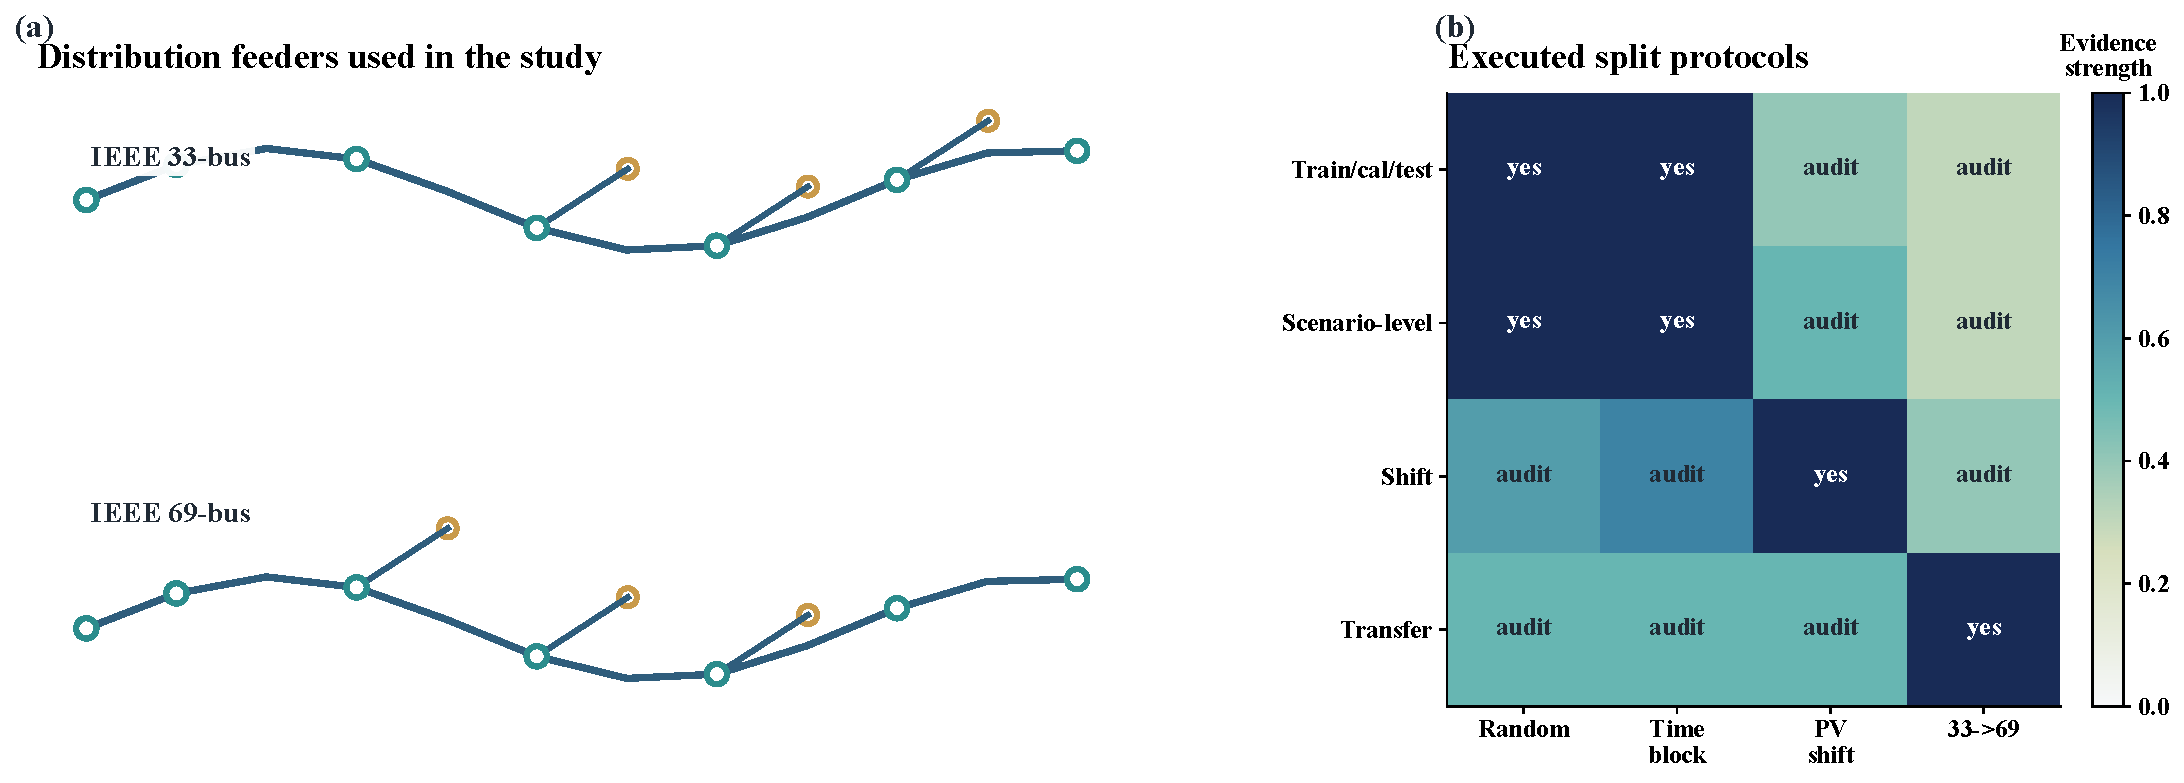
\includegraphics[width=1.1\linewidth,height=\textheight,keepaspectratio,alt={Main distribution feeders and generalization protocols. (a) IEEE 33-bus and 69-bus distribution feeders used as the main experimental systems; (b) executed split protocols for random interpolation, synthetic time-block, PV-shift, and topology-transfer audits.}]{figures/fig02_feeders_and_splits.pdf}
\caption{Main distribution feeders and generalization protocols. (a)
IEEE 33-bus and 69-bus distribution feeders used as the main
experimental systems; (b) executed split protocols for random
interpolation, synthetic time-block, PV-shift, and topology-transfer
audits.}\label{fig:fig02_feeders_and_splits}
\end{figure}

\section{Results}\label{results}

\subsection{Representative Random-Split
Results}\label{representative-random-split-results}

On the representative IEEE 33/69 random split, VoltGuard with
topology+PV+loading conditioned calibration achieves the strongest
screening tradeoff among the selected main estimators.

{\def\LTcaptype{none} % do not increment counter
\begin{longtable}[]{@{}
  >{\raggedright\arraybackslash}p{(\linewidth - 14\tabcolsep) * \real{0.1000}}
  >{\raggedright\arraybackslash}p{(\linewidth - 14\tabcolsep) * \real{0.1000}}
  >{\raggedleft\arraybackslash}p{(\linewidth - 14\tabcolsep) * \real{0.1333}}
  >{\raggedleft\arraybackslash}p{(\linewidth - 14\tabcolsep) * \real{0.1333}}
  >{\raggedleft\arraybackslash}p{(\linewidth - 14\tabcolsep) * \real{0.1333}}
  >{\raggedleft\arraybackslash}p{(\linewidth - 14\tabcolsep) * \real{0.1333}}
  >{\raggedleft\arraybackslash}p{(\linewidth - 14\tabcolsep) * \real{0.1333}}
  >{\raggedleft\arraybackslash}p{(\linewidth - 14\tabcolsep) * \real{0.1333}}@{}}
\toprule\noalign{}
\begin{minipage}[b]{\linewidth}\raggedright
Method
\end{minipage} & \begin{minipage}[b]{\linewidth}\raggedright
Conformal variant
\end{minipage} & \begin{minipage}[b]{\linewidth}\raggedleft
RMSE
\end{minipage} & \begin{minipage}[b]{\linewidth}\raggedleft
Coverage
\end{minipage} & \begin{minipage}[b]{\linewidth}\raggedleft
Width
\end{minipage} & \begin{minipage}[b]{\linewidth}\raggedleft
Recall
\end{minipage} & \begin{minipage}[b]{\linewidth}\raggedleft
False alarm
\end{minipage} & \begin{minipage}[b]{\linewidth}\raggedleft
Missed
\end{minipage} \\
\midrule\noalign{}
\endhead
\bottomrule\noalign{}
\endlastfoot
LinDistFlow physical backbone & none & 0.00140 & -- & -- & 0.91640 &
0.00000 & 77 \\
Random forest & none & 0.00023 & -- & -- & 0.99023 & 0.00019 & 9 \\
Gradient boosting & none & 0.00041 & -- & -- & 0.97286 & 0.00000 & 25 \\
Boosting point + global conformal & global & 0.00041 & 0.90850 & 0.00110
& 0.99674 & 0.00250 & 3 \\
VoltGuard topology-aware residual & topology+PV+loading & 0.00011 &
0.93660 & 0.00043 & 0.99891 & 0.00058 & 1 \\
Neural graph residual ablation & topology & 0.00171 & 0.91340 & 0.00540
& 0.99783 & 0.02327 & 2 \\
\end{longtable}
}

The neural ablation attains high recall but with substantially wider
intervals, higher RMSE, and higher false-alarm rate. It is therefore
kept as an ablation, not as the main estimator.

\subsection{Branch-Level Physics Consistency
Audit}\label{branch-level-physics-consistency-audit}

Because VoltGuard corrects a LinDistFlow-style voltage proxy, we audit
whether the saved voltage predictions remain consistent with the
branch-level voltage-drop relation used in the methodology. For each
representative test scenario, feeder branches are oriented from the
slack bus, downstream forecast net injections are aggregated, and the
residual

\[
\hat u_j-\hat u_i+2(r_{ij}\hat P_{ij}+x_{ij}\hat Q_{ij})
\]

is computed on each branch. This is a LinDistFlow consistency audit, not
an AC feasibility certificate; the AC-label row is not zero because the
proxy ignores losses and other full AC effects.

{\def\LTcaptype{none} % do not increment counter
\begin{longtable}[]{@{}
  >{\raggedright\arraybackslash}p{(\linewidth - 12\tabcolsep) * \real{0.1154}}
  >{\raggedright\arraybackslash}p{(\linewidth - 12\tabcolsep) * \real{0.1154}}
  >{\raggedleft\arraybackslash}p{(\linewidth - 12\tabcolsep) * \real{0.1538}}
  >{\raggedleft\arraybackslash}p{(\linewidth - 12\tabcolsep) * \real{0.1538}}
  >{\raggedleft\arraybackslash}p{(\linewidth - 12\tabcolsep) * \real{0.1538}}
  >{\raggedleft\arraybackslash}p{(\linewidth - 12\tabcolsep) * \real{0.1538}}
  >{\raggedleft\arraybackslash}p{(\linewidth - 12\tabcolsep) * \real{0.1538}}@{}}
\toprule\noalign{}
\begin{minipage}[b]{\linewidth}\raggedright
Method
\end{minipage} & \begin{minipage}[b]{\linewidth}\raggedright
Variant
\end{minipage} & \begin{minipage}[b]{\linewidth}\raggedleft
Scenarios
\end{minipage} & \begin{minipage}[b]{\linewidth}\raggedleft
Drop RMSE
\end{minipage} & \begin{minipage}[b]{\linewidth}\raggedleft
Drop MAE
\end{minipage} & \begin{minipage}[b]{\linewidth}\raggedleft
95\% max-abs drop residual
\end{minipage} & \begin{minipage}[b]{\linewidth}\raggedleft
Violating-only drop RMSE
\end{minipage} \\
\midrule\noalign{}
\endhead
\bottomrule\noalign{}
\endlastfoot
AC power-flow label & reference & 120 & 0.000238 & 0.000101 & 0.002516 &
0.000272 \\
Boosting point + global conformal & global & 120 & 0.000563 & 0.000379 &
0.004631 & 0.000621 \\
VoltGuard topology-aware residual & topology+PV+loading & 120 & 0.000250
& 0.000122 & 0.002395 & 0.000279 \\
Neural graph residual ablation & topology & 120 & 0.003139 & 0.002437 &
0.014201 & 0.002904 \\
\end{longtable}
}

VoltGuard substantially reduces the branch-drop RMSE relative to
boosting plus global conformal and remains close to the AC-label audit
residual, while the neural graph residual is substantially less
consistent with the LinDistFlow drop relation. This supports the paper's
physics-informed claim in the narrow sense used here: residual learning
is anchored to a real LinDistFlow backbone, operating features, and
topology in a way that improves calibrated screening without moving far
from the physical voltage-drop structure.

\subsection{Multi-Seed Random-Split
Statistics}\label{multi-seed-random-split-statistics}

Across three random seeds, VoltGuard reduces missed violations relative
to boosting plus global conformal while maintaining near-nominal
coverage.

{\def\LTcaptype{none} % do not increment counter
\begin{longtable}[]{@{}
  >{\raggedright\arraybackslash}p{(\linewidth - 16\tabcolsep) * \real{0.0882}}
  >{\raggedright\arraybackslash}p{(\linewidth - 16\tabcolsep) * \real{0.0882}}
  >{\raggedleft\arraybackslash}p{(\linewidth - 16\tabcolsep) * \real{0.1176}}
  >{\raggedleft\arraybackslash}p{(\linewidth - 16\tabcolsep) * \real{0.1176}}
  >{\raggedleft\arraybackslash}p{(\linewidth - 16\tabcolsep) * \real{0.1176}}
  >{\raggedleft\arraybackslash}p{(\linewidth - 16\tabcolsep) * \real{0.1176}}
  >{\raggedleft\arraybackslash}p{(\linewidth - 16\tabcolsep) * \real{0.1176}}
  >{\raggedleft\arraybackslash}p{(\linewidth - 16\tabcolsep) * \real{0.1176}}
  >{\raggedleft\arraybackslash}p{(\linewidth - 16\tabcolsep) * \real{0.1176}}@{}}
\toprule\noalign{}
\begin{minipage}[b]{\linewidth}\raggedright
Method
\end{minipage} & \begin{minipage}[b]{\linewidth}\raggedright
Variant
\end{minipage} & \begin{minipage}[b]{\linewidth}\raggedleft
RMSE mean
\end{minipage} & \begin{minipage}[b]{\linewidth}\raggedleft
Coverage mean
\end{minipage} & \begin{minipage}[b]{\linewidth}\raggedleft
Width mean
\end{minipage} & \begin{minipage}[b]{\linewidth}\raggedleft
Recall mean
\end{minipage} & \begin{minipage}[b]{\linewidth}\raggedleft
False alarm mean
\end{minipage} & \begin{minipage}[b]{\linewidth}\raggedleft
Missed mean
\end{minipage} & \begin{minipage}[b]{\linewidth}\raggedleft
Runs
\end{minipage} \\
\midrule\noalign{}
\endhead
\bottomrule\noalign{}
\endlastfoot
Boosting point + global conformal & global & 0.00076 & 0.90468 & 0.00127
& 0.99811 & 0.00240 & 1.67 & 3 \\
VoltGuard topology-aware residual & topology+PV+loading & 0.00017 &
0.92397 & 0.00049 & 0.99964 & 0.00171 & 0.33 & 3 \\
\end{longtable}
}

The confidence intervals are reported in
\texttt{multi\_seed\_summary.md}. The main interpretation is not that
every seed dominates on every metric, but that conditioned calibration
improves the risk-recall tradeoff without relying on a GNN claim.

We also report paired seed deltas relative to boosting plus global
conformal, using the same split seed before averaging. Positive deltas
mean VoltGuard is larger; negative deltas are better for RMSE, width,
false alarms, and missed violations. On the random interpolation split,
VoltGuard reduces missed bus-level violations by 1.33 on average,
increases recall by 0.00152, and narrows intervals by 0.00078 p.u. On
synthetic time-block splits, the paired missed-violation reduction is
also 1.33. Under PV-shift, VoltGuard keeps recall slightly higher while
coverage drops below nominal, reflecting the deliberately shifted test
distribution. Under topology-held-out 33-to-69 transfer, missed
violations are unchanged while intervals and false alarms are lower, but
this is still a protocol-specific transfer result rather than a
topology-invariant safety guarantee.

{\def\LTcaptype{none} % do not increment counter
\begin{longtable}[]{@{}
  >{\raggedright\arraybackslash}p{(\linewidth - 12\tabcolsep) * \real{0.1111}}
  >{\raggedleft\arraybackslash}p{(\linewidth - 12\tabcolsep) * \real{0.1481}}
  >{\raggedleft\arraybackslash}p{(\linewidth - 12\tabcolsep) * \real{0.1481}}
  >{\raggedleft\arraybackslash}p{(\linewidth - 12\tabcolsep) * \real{0.1481}}
  >{\raggedleft\arraybackslash}p{(\linewidth - 12\tabcolsep) * \real{0.1481}}
  >{\raggedleft\arraybackslash}p{(\linewidth - 12\tabcolsep) * \real{0.1481}}
  >{\raggedleft\arraybackslash}p{(\linewidth - 12\tabcolsep) * \real{0.1481}}@{}}
\toprule\noalign{}
\begin{minipage}[b]{\linewidth}\raggedright
Split
\end{minipage} & \begin{minipage}[b]{\linewidth}\raggedleft
Runs
\end{minipage} & \begin{minipage}[b]{\linewidth}\raggedleft
Delta coverage
\end{minipage} & \begin{minipage}[b]{\linewidth}\raggedleft
Delta width
\end{minipage} & \begin{minipage}[b]{\linewidth}\raggedleft
Delta recall
\end{minipage} & \begin{minipage}[b]{\linewidth}\raggedleft
Delta false alarm
\end{minipage} & \begin{minipage}[b]{\linewidth}\raggedleft
Delta missed
\end{minipage} \\
\midrule\noalign{}
\endhead
\bottomrule\noalign{}
\endlastfoot
random interpolation & 3 & 0.01928 & -0.00078 & 0.00152 & -0.00070 &
-1.33 \\
synthetic time-block & 3 & 0.04025 & -0.00058 & 0.00140 & -0.00110 &
-1.33 \\
PV-penetration shift & 3 & -0.02652 & -0.00044 & 0.00064 & -0.00016 &
-0.33 \\
topology-held-out 33-to-69 & 3 & 0.00242 & -0.00078 & 0.00000 & -0.00129
& 0.00 \\
\end{longtable}
}

\subsection{Feature/Residual Ablation}\label{featureresidual-ablation}

We add a feature/residual ablation to test whether the main estimator is
actually topology-aware or merely a generic tree ensemble. All variants
use the same topology/PV/loading conformal calibration and three random
seeds. The local-only residual learner uses only bus-level operating
quantities; the local+topology variant adds bus position, voltage base,
degree, slack indicator, and feeder code; the full variant also includes
neighbor load/PV/net-demand features. A direct full ExtraTrees model
tests whether the residual formulation matters once the same full
feature family is available.

{\def\LTcaptype{none} % do not increment counter
\begin{longtable}[]{@{}
  >{\raggedright\arraybackslash}p{(\linewidth - 16\tabcolsep) * \real{0.0882}}
  >{\raggedright\arraybackslash}p{(\linewidth - 16\tabcolsep) * \real{0.0882}}
  >{\raggedleft\arraybackslash}p{(\linewidth - 16\tabcolsep) * \real{0.1176}}
  >{\raggedleft\arraybackslash}p{(\linewidth - 16\tabcolsep) * \real{0.1176}}
  >{\raggedleft\arraybackslash}p{(\linewidth - 16\tabcolsep) * \real{0.1176}}
  >{\raggedleft\arraybackslash}p{(\linewidth - 16\tabcolsep) * \real{0.1176}}
  >{\raggedleft\arraybackslash}p{(\linewidth - 16\tabcolsep) * \real{0.1176}}
  >{\raggedleft\arraybackslash}p{(\linewidth - 16\tabcolsep) * \real{0.1176}}
  >{\raggedleft\arraybackslash}p{(\linewidth - 16\tabcolsep) * \real{0.1176}}@{}}
\toprule\noalign{}
\begin{minipage}[b]{\linewidth}\raggedright
Variant
\end{minipage} & \begin{minipage}[b]{\linewidth}\raggedright
Feature family
\end{minipage} & \begin{minipage}[b]{\linewidth}\raggedleft
Runs
\end{minipage} & \begin{minipage}[b]{\linewidth}\raggedleft
RMSE
\end{minipage} & \begin{minipage}[b]{\linewidth}\raggedleft
Coverage
\end{minipage} & \begin{minipage}[b]{\linewidth}\raggedleft
Width
\end{minipage} & \begin{minipage}[b]{\linewidth}\raggedleft
Recall
\end{minipage} & \begin{minipage}[b]{\linewidth}\raggedleft
False alarm
\end{minipage} & \begin{minipage}[b]{\linewidth}\raggedleft
Missed
\end{minipage} \\
\midrule\noalign{}
\endhead
\bottomrule\noalign{}
\endlastfoot
direct & full topology/electrical & 3 & 0.00029 & 0.91111 & 0.00073 &
0.99848 & 0.00298 & 1.33 \\
residual & local operating only & 3 & 0.00073 & 0.92195 & 0.00207 &
0.99621 & 0.00373 & 3.33 \\
residual & local+topology & 3 & 0.00022 & 0.91694 & 0.00071 & 0.99964 &
0.00298 & 0.33 \\
residual & full topology/electrical & 3 & 0.00017 & 0.92413 & 0.00050 &
0.99964 & 0.00171 & 0.33 \\
\end{longtable}
}

The ablation supports the topology/electrical part of the claim
strongly: removing topology and neighbor electrical features increases
the mean missed bus-level violations from 0.33 to 3.33 and widens
intervals from 0.00050 to 0.00207 p.u. The residual formulation should
be read more narrowly. Relative to a direct full ExtraTrees predictor,
the residual full model lowers RMSE (0.00017 versus 0.00029), interval
width (0.00050 versus 0.00073), and false-alarm rate (0.00171 versus
0.00298), while both the full residual and local+topology residual have
statistically comparable missed-violation counts. This is why the paper
emphasizes physics-informed topology-aware residual screening rather
than claiming that residualization alone dominates every operating
metric.

\subsection{Comparison with Competing Screening
Methods}\label{comparison-with-competing-screening-methods}

The reviewer-requested comparison table brings together the
representative random-split results for physical, tree-based, conformal,
statistical-UQ, and graph-residual screens. The quantile-regression and
Gaussian-process rows are additional baselines run on the same seed-7
random split. The Gaussian-process baseline uses a 900-row training
subsample for tractability and is included to test whether generic
probabilistic regression gives useful screening intervals without
feeder-specific residual structure.

{\def\LTcaptype{none} % do not increment counter
\begin{longtable}[]{@{}
  >{\raggedright\arraybackslash}p{(\linewidth - 14\tabcolsep) * \real{0.1000}}
  >{\raggedright\arraybackslash}p{(\linewidth - 14\tabcolsep) * \real{0.1000}}
  >{\raggedleft\arraybackslash}p{(\linewidth - 14\tabcolsep) * \real{0.1333}}
  >{\raggedleft\arraybackslash}p{(\linewidth - 14\tabcolsep) * \real{0.1333}}
  >{\raggedleft\arraybackslash}p{(\linewidth - 14\tabcolsep) * \real{0.1333}}
  >{\raggedleft\arraybackslash}p{(\linewidth - 14\tabcolsep) * \real{0.1333}}
  >{\raggedleft\arraybackslash}p{(\linewidth - 14\tabcolsep) * \real{0.1333}}
  >{\raggedleft\arraybackslash}p{(\linewidth - 14\tabcolsep) * \real{0.1333}}@{}}
\toprule\noalign{}
\begin{minipage}[b]{\linewidth}\raggedright
Method
\end{minipage} & \begin{minipage}[b]{\linewidth}\raggedright
Interval source
\end{minipage} & \begin{minipage}[b]{\linewidth}\raggedleft
RMSE
\end{minipage} & \begin{minipage}[b]{\linewidth}\raggedleft
Coverage
\end{minipage} & \begin{minipage}[b]{\linewidth}\raggedleft
Width
\end{minipage} & \begin{minipage}[b]{\linewidth}\raggedleft
Recall
\end{minipage} & \begin{minipage}[b]{\linewidth}\raggedleft
False alarm
\end{minipage} & \begin{minipage}[b]{\linewidth}\raggedleft
Missed
\end{minipage} \\
\midrule\noalign{}
\endhead
\bottomrule\noalign{}
\endlastfoot
LinDistFlow physical backbone & point only & 0.00140 & n/a & n/a &
0.91640 & 0.00000 & 77 \\
Random forest & point only & 0.00023 & n/a & n/a & 0.99023 & 0.00019 &
9 \\
Gradient boosting & point only & 0.00042 & n/a & n/a & 0.97286 & 0.00000
& 25 \\
Boosting + global conformal & pooled residual quantile & 0.00042 &
0.90850 & 0.00110 & 0.99674 & 0.00250 & 3 \\
Gradient-boosted quantile regression & learned 5/95\% quantiles &
0.00035 & 0.83219 & 0.00444 & 0.99566 & 0.00135 & 4 \\
Gaussian-process UQ baseline & 90\% Gaussian interval & 0.01165 &
0.97827 & 0.05108 & 1.00000 & 0.33353 & 0 \\
Neural graph residual ablation & topology conformal & 0.00171 & 0.91340
& 0.00540 & 0.99783 & 0.02327 & 2 \\
VoltGuard topology-aware residual & topology/PV/loading conformal &
0.00011 & 0.93660 & 0.00043 & 0.99891 & 0.00058 & 1 \\
\end{longtable}
}

The comparison clarifies the novelty boundary. Standard tree models can
give competitive point accuracy, but their uncalibrated risk flags miss
more violations. Global conformal calibration improves recall but is
less sharp than conditioned calibration. Quantile regression gives
intervals but under-covers in this split, while generic Gaussian-process
intervals become too wide and produce many false alarms. The graph
residual does not outperform the topology-aware residual learner.
VoltGuard's advantage is therefore the combination of a physical voltage
proxy, topology/electrical residual features, and conditioned conformal
calibration rather than a generic ML model alone.

\subsection{Conformal Ablation}\label{conformal-ablation}

The representative random split directly compares calibration variants.

{\def\LTcaptype{none} % do not increment counter
\begin{longtable}[]{@{}
  >{\raggedright\arraybackslash}p{(\linewidth - 10\tabcolsep) * \real{0.1304}}
  >{\raggedleft\arraybackslash}p{(\linewidth - 10\tabcolsep) * \real{0.1739}}
  >{\raggedleft\arraybackslash}p{(\linewidth - 10\tabcolsep) * \real{0.1739}}
  >{\raggedleft\arraybackslash}p{(\linewidth - 10\tabcolsep) * \real{0.1739}}
  >{\raggedleft\arraybackslash}p{(\linewidth - 10\tabcolsep) * \real{0.1739}}
  >{\raggedleft\arraybackslash}p{(\linewidth - 10\tabcolsep) * \real{0.1739}}@{}}
\toprule\noalign{}
\begin{minipage}[b]{\linewidth}\raggedright
Variant
\end{minipage} & \begin{minipage}[b]{\linewidth}\raggedleft
Coverage
\end{minipage} & \begin{minipage}[b]{\linewidth}\raggedleft
Width
\end{minipage} & \begin{minipage}[b]{\linewidth}\raggedleft
Recall
\end{minipage} & \begin{minipage}[b]{\linewidth}\raggedleft
False alarm
\end{minipage} & \begin{minipage}[b]{\linewidth}\raggedleft
Missed
\end{minipage} \\
\midrule\noalign{}
\endhead
\bottomrule\noalign{}
\endlastfoot
global & 0.94984 & 0.00053 & 0.99891 & 0.00115 & 1 \\
PV-conditioned & 0.94510 & 0.00049 & 0.99891 & 0.00058 & 1 \\
topology-conditioned & 0.95523 & 0.00053 & 0.99891 & 0.00154 & 1 \\
topology+PV+loading conditioned & 0.93660 & 0.00043 & 0.99891 & 0.00058
& 1 \\
topology+PV+loading no-shrinkage & 0.91258 & 0.00042 & 0.99891 & 0.00038
& 1 \\
\end{longtable}
}

All VoltGuard conformal variants miss only one bus-level violation in
this split. The topology+PV+loading conditioned variant is selected
because it keeps that recall while producing the sharpest
shrinkage-stabilized interval; the no-shrinkage version is marginally
narrower but loses coverage, which is why shrinkage remains in the main
method.

\begin{figure}
\centering
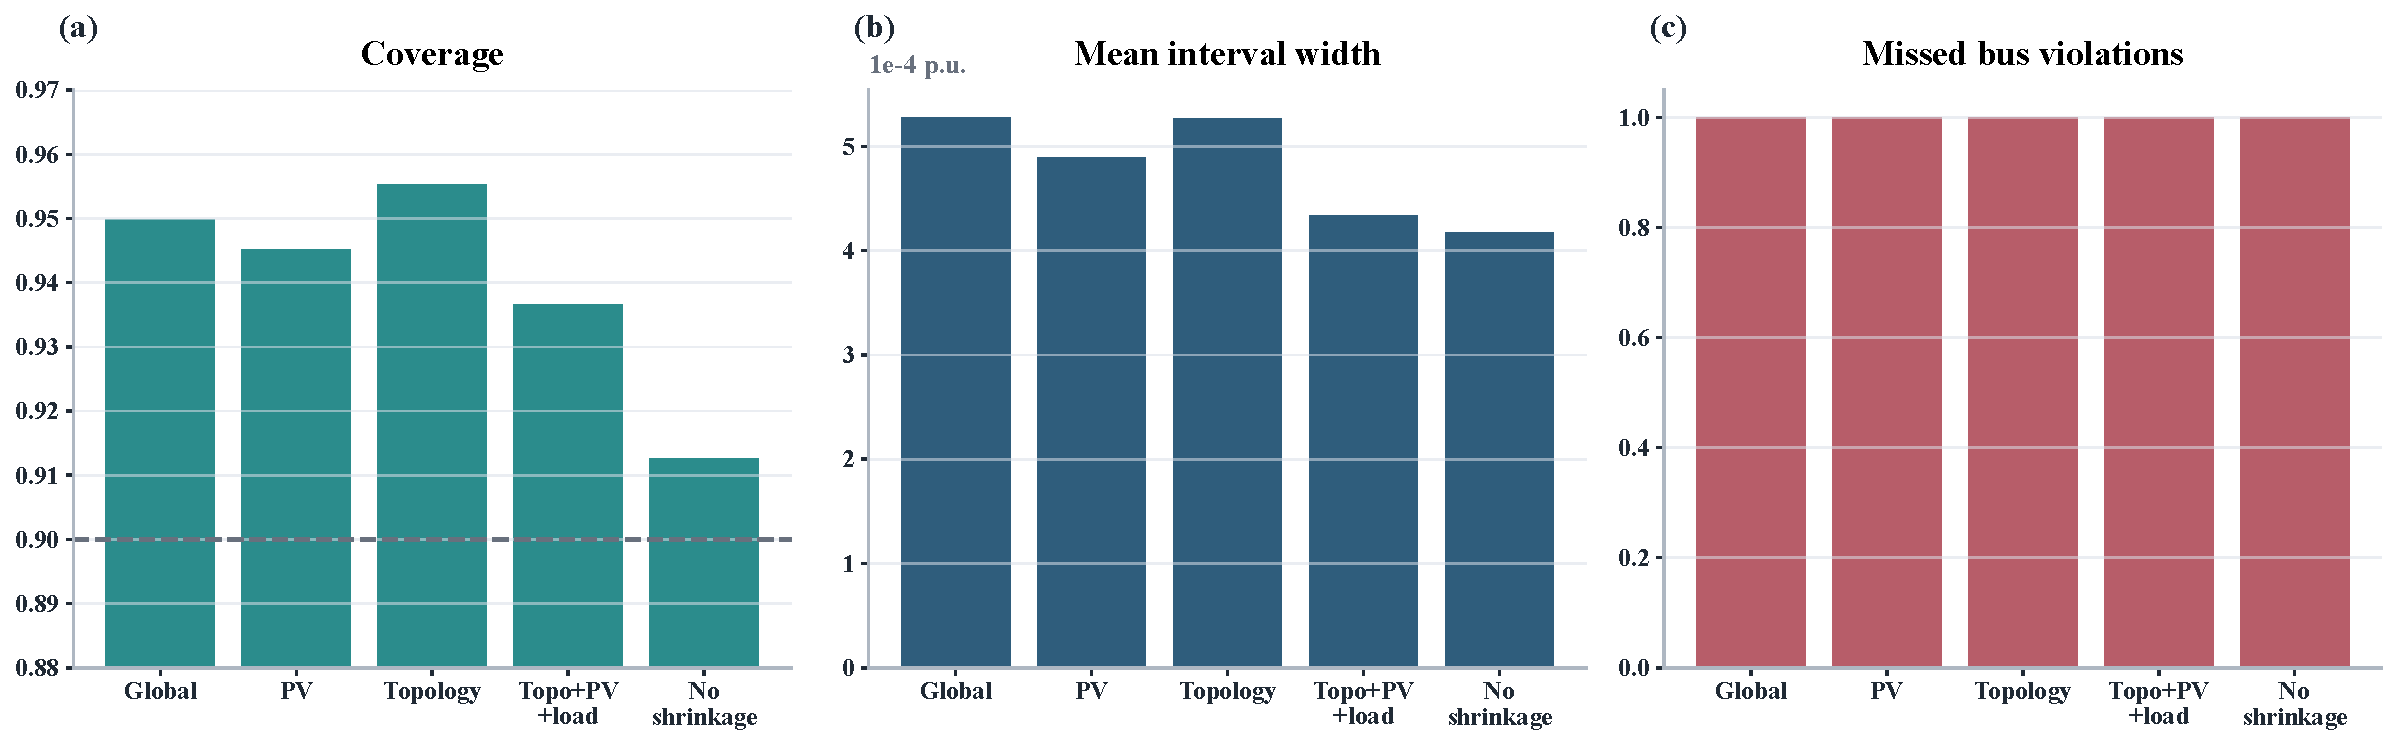
\includegraphics[width=1.1\linewidth,height=\textheight,keepaspectratio,alt={Conformal calibration variant comparison. (a) Empirical coverage across calibration variants; (b) mean interval width; (c) missed bus-level voltage violations.}]{figures/fig03_conformal_ablation.pdf}
\caption{Conformal calibration variant comparison. (a) Empirical
coverage across calibration variants; (b) mean interval width; (c)
missed bus-level voltage
violations.}\label{fig:fig03_conformal_ablation}
\end{figure}

\subsection{Calibration-Budget
Sensitivity}\label{calibration-budget-sensitivity}

Conditioned conformal calibration is useful only if the calibration set
covers the operating families that will appear at test time. We
therefore add a scenario-level calibration-budget audit using the saved
representative split. The residual model is not retrained. Instead,
calibration scenarios are sampled without replacement at 10\%, 25\%,
50\%, 75\%, and 100\% of the calibration split, and conformal radii are
recomputed before evaluating the same held-out test set. Partial-budget
cases are repeated 20 times. Sampling is done at the scenario level so
buses from the same scenario are not treated as independent calibration
draws.

{\def\LTcaptype{none} % do not increment counter
\begin{longtable}[]{@{}
  >{\raggedright\arraybackslash}p{(\linewidth - 18\tabcolsep) * \real{0.0769}}
  >{\raggedleft\arraybackslash}p{(\linewidth - 18\tabcolsep) * \real{0.1026}}
  >{\raggedleft\arraybackslash}p{(\linewidth - 18\tabcolsep) * \real{0.1026}}
  >{\raggedleft\arraybackslash}p{(\linewidth - 18\tabcolsep) * \real{0.1026}}
  >{\raggedleft\arraybackslash}p{(\linewidth - 18\tabcolsep) * \real{0.1026}}
  >{\raggedleft\arraybackslash}p{(\linewidth - 18\tabcolsep) * \real{0.1026}}
  >{\raggedleft\arraybackslash}p{(\linewidth - 18\tabcolsep) * \real{0.1026}}
  >{\raggedleft\arraybackslash}p{(\linewidth - 18\tabcolsep) * \real{0.1026}}
  >{\raggedleft\arraybackslash}p{(\linewidth - 18\tabcolsep) * \real{0.1026}}
  >{\raggedleft\arraybackslash}p{(\linewidth - 18\tabcolsep) * \real{0.1026}}@{}}
\toprule\noalign{}
\begin{minipage}[b]{\linewidth}\raggedright
Method
\end{minipage} & \begin{minipage}[b]{\linewidth}\raggedleft
Calib. fraction
\end{minipage} & \begin{minipage}[b]{\linewidth}\raggedleft
Calib. scenarios
\end{minipage} & \begin{minipage}[b]{\linewidth}\raggedleft
Observed families
\end{minipage} & \begin{minipage}[b]{\linewidth}\raggedleft
Empty test families
\end{minipage} & \begin{minipage}[b]{\linewidth}\raggedleft
Coverage
\end{minipage} & \begin{minipage}[b]{\linewidth}\raggedleft
Width
\end{minipage} & \begin{minipage}[b]{\linewidth}\raggedleft
Recall
\end{minipage} & \begin{minipage}[b]{\linewidth}\raggedleft
False alarm
\end{minipage} & \begin{minipage}[b]{\linewidth}\raggedleft
Missed
\end{minipage} \\
\midrule\noalign{}
\endhead
\bottomrule\noalign{}
\endlastfoot
Boosting + global & 0.10 & 12 & 1.00 & 0.00 & 0.89410 & 0.00104 &
0.99457 & 0.00181 & 5.00 \\
Boosting + global & 1.00 & 120 & 1.00 & 0.00 & 0.90850 & 0.00110 &
0.99674 & 0.00250 & 3.00 \\
VoltGuard topology+PV+loading & 0.10 & 12 & 8.40 & 7.60 & 0.92903 &
0.00047 & 0.99902 & 0.00110 & 0.90 \\
VoltGuard topology+PV+loading & 0.25 & 30 & 13.35 & 2.65 & 0.93528 &
0.00044 & 0.99924 & 0.00091 & 0.70 \\
VoltGuard topology+PV+loading & 0.50 & 60 & 15.80 & 0.20 & 0.94022 &
0.00044 & 0.99919 & 0.00089 & 0.75 \\
VoltGuard topology+PV+loading & 0.75 & 90 & 16.00 & 0.00 & 0.94051 &
0.00044 & 0.99919 & 0.00078 & 0.75 \\
VoltGuard topology+PV+loading & 1.00 & 120 & 16.00 & 0.00 & 0.93660 &
0.00043 & 0.99891 & 0.00058 & 1.00 \\
\end{longtable}
}

The budget audit supports deployment, but with a clear boundary. With
only 12 calibration scenarios, the shrinkage/fallback construction
prevents the screen from collapsing: coverage remains 0.92903 and the
mean missed bus-level violations stay below one in this representative
test set. However, the calibration set observes only 8.4 of the 16 test
families on average, so many conditioned families are not actually
calibrated locally. At 75\% and full budget, all 16 families are
observed. We therefore describe small-budget results as evidence for a
robust fallback mechanism, not as evidence for family-wise coverage
without family-level calibration diversity.

\subsection{Asymmetric Conformal
Audit}\label{asymmetric-conformal-audit}

We also audit an asymmetric one-sided conformal variant because voltage
limits are directional: undervoltage risk depends on the lower tail and
overvoltage risk depends on the upper tail. This audit uses the same
saved calibration and test predictions and replaces the symmetric
absolute-residual radius with separate lower and upper one-sided
conformal radii. It is not a new distribution-shift guarantee; it is a
tail-aware calibration ablation under the same split and exchangeability
assumptions as the main conformal analysis.

{\def\LTcaptype{none} % do not increment counter
\begin{longtable}[]{@{}
  >{\raggedright\arraybackslash}p{(\linewidth - 12\tabcolsep) * \real{0.1154}}
  >{\raggedright\arraybackslash}p{(\linewidth - 12\tabcolsep) * \real{0.1154}}
  >{\raggedleft\arraybackslash}p{(\linewidth - 12\tabcolsep) * \real{0.1538}}
  >{\raggedleft\arraybackslash}p{(\linewidth - 12\tabcolsep) * \real{0.1538}}
  >{\raggedleft\arraybackslash}p{(\linewidth - 12\tabcolsep) * \real{0.1538}}
  >{\raggedleft\arraybackslash}p{(\linewidth - 12\tabcolsep) * \real{0.1538}}
  >{\raggedleft\arraybackslash}p{(\linewidth - 12\tabcolsep) * \real{0.1538}}@{}}
\toprule\noalign{}
\begin{minipage}[b]{\linewidth}\raggedright
Method
\end{minipage} & \begin{minipage}[b]{\linewidth}\raggedright
Calibration
\end{minipage} & \begin{minipage}[b]{\linewidth}\raggedleft
Coverage
\end{minipage} & \begin{minipage}[b]{\linewidth}\raggedleft
Width
\end{minipage} & \begin{minipage}[b]{\linewidth}\raggedleft
Recall
\end{minipage} & \begin{minipage}[b]{\linewidth}\raggedleft
False alarm
\end{minipage} & \begin{minipage}[b]{\linewidth}\raggedleft
Missed
\end{minipage} \\
\midrule\noalign{}
\endhead
\bottomrule\noalign{}
\endlastfoot
Boosting + global conformal & symmetric & 0.90850 & 0.001096 & 0.99674 &
0.00250 & 3 \\
Boosting + global conformal & asymmetric & 0.90539 & 0.001162 & 0.99891
& 0.00327 & 1 \\
VoltGuard global & symmetric & 0.94984 & 0.000527 & 0.99891 & 0.00115 &
1 \\
VoltGuard global & asymmetric & 0.94624 & 0.000497 & 0.99891 & 0.00058 &
1 \\
VoltGuard topology+PV+loading & symmetric & 0.93660 & 0.000433 & 0.99891
& 0.00058 & 1 \\
VoltGuard topology+PV+loading & asymmetric & 0.91977 & 0.000411 &
1.00000 & 0.00058 & 0 \\
\end{longtable}
}

For the main topology+PV+loading variant, the asymmetric audit narrows
the mean interval by 0.000022 p.u. and removes the remaining missed
bus-level violation while retaining scenario-level recall of 1.0. The
cost is lower empirical coverage, 0.91977 rather than 0.93660, although
still above the nominal 90\% target in this representative split. We
therefore keep symmetric conditioned conformal calibration as the main
method and report the asymmetric variant as an optional tail-aware
extension that may be useful when missed voltage violations are costlier
than modest interval-efficiency loss.

\subsection{EV-Conditioning Ablation}\label{ev-conditioning-ablation}

Because the scenarios also include EV charging perturbations, we add an
EV-conditioned ablation to test whether EV scale should be added to the
conformal family key. The result is negative for the current sample
size. Adding EV to the topology+PV+loading family increases the number
of families from 16 to 55, reduces the minimum calibration count from
198 to 33, and leaves seven empty test families. It does not reduce
missed violations or improve recall; it increases interval width and
false alarms. Thus EV demand remains a pre-dispatch feature for residual
learning, but the conformal calibration key is kept at feeder/PV/loading
granularity unless a larger EV-calibration set is available.

{\def\LTcaptype{none} % do not increment counter
\begin{longtable}[]{@{}
  >{\raggedright\arraybackslash}p{(\linewidth - 16\tabcolsep) * \real{0.0857}}
  >{\raggedleft\arraybackslash}p{(\linewidth - 16\tabcolsep) * \real{0.1143}}
  >{\raggedleft\arraybackslash}p{(\linewidth - 16\tabcolsep) * \real{0.1143}}
  >{\raggedleft\arraybackslash}p{(\linewidth - 16\tabcolsep) * \real{0.1143}}
  >{\raggedleft\arraybackslash}p{(\linewidth - 16\tabcolsep) * \real{0.1143}}
  >{\raggedleft\arraybackslash}p{(\linewidth - 16\tabcolsep) * \real{0.1143}}
  >{\raggedleft\arraybackslash}p{(\linewidth - 16\tabcolsep) * \real{0.1143}}
  >{\raggedleft\arraybackslash}p{(\linewidth - 16\tabcolsep) * \real{0.1143}}
  >{\raggedleft\arraybackslash}p{(\linewidth - 16\tabcolsep) * \real{0.1143}}@{}}
\toprule\noalign{}
\begin{minipage}[b]{\linewidth}\raggedright
Conditioning key
\end{minipage} & \begin{minipage}[b]{\linewidth}\raggedleft
Families
\end{minipage} & \begin{minipage}[b]{\linewidth}\raggedleft
Min calib.
\end{minipage} & \begin{minipage}[b]{\linewidth}\raggedleft
Empty test families
\end{minipage} & \begin{minipage}[b]{\linewidth}\raggedleft
Coverage
\end{minipage} & \begin{minipage}[b]{\linewidth}\raggedleft
Width
\end{minipage} & \begin{minipage}[b]{\linewidth}\raggedleft
Recall
\end{minipage} & \begin{minipage}[b]{\linewidth}\raggedleft
False alarm
\end{minipage} & \begin{minipage}[b]{\linewidth}\raggedleft
Missed
\end{minipage} \\
\midrule\noalign{}
\endhead
\bottomrule\noalign{}
\endlastfoot
topology+PV+loading & 16 & 198 & 0 & 0.93660 & 0.00043 & 0.99891 &
0.00058 & 1 \\
topology+PV+loading+EV & 55 & 33 & 7 & 0.94918 & 0.00048 & 0.99891 &
0.00154 & 1 \\
topology+PV+EV & 31 & 33 & 1 & 0.94853 & 0.00050 & 0.99891 & 0.00173 &
1 \\
PV+loading+EV & 32 & 33 & 0 & 0.94003 & 0.00045 & 0.99891 & 0.00077 &
1 \\
EV-only & 4 & 1359 & 0 & 0.94444 & 0.00053 & 0.99891 & 0.00115 & 1 \\
\end{longtable}
}

This ablation is therefore a sample-size outlook rather than a claim
that EV information has no value. At the current calibration scale, EV
bins fragment the calibration set: the most detailed EV-conditioned key
has only 33 samples in its smallest calibration family, compared with
198 for the primary topology+PV+loading key. If the same scenario design
were expanded while keeping the EV family definition fixed, the
EV-conditioned split would need roughly six times more calibration
support before its weakest family matches the primary grouping. The
supplementary sensitivity curve below records this threshold logic and
should be used to decide when EV-conditioned calibration is worth
retesting.

{\def\LTcaptype{none} % do not increment counter
\begin{longtable}[]{@{}
  >{\raggedleft\arraybackslash}p{(\linewidth - 4\tabcolsep) * \real{0.3636}}
  >{\raggedleft\arraybackslash}p{(\linewidth - 4\tabcolsep) * \real{0.3636}}
  >{\raggedright\arraybackslash}p{(\linewidth - 4\tabcolsep) * \real{0.2727}}@{}}
\toprule\noalign{}
\begin{minipage}[b]{\linewidth}\raggedleft
Calibration scale relative to current EV-conditioned split
\end{minipage} & \begin{minipage}[b]{\linewidth}\raggedleft
Approx. minimum EV-family calibration samples
\end{minipage} & \begin{minipage}[b]{\linewidth}\raggedright
Expected EV-conditioning status
\end{minipage} \\
\midrule\noalign{}
\endhead
\bottomrule\noalign{}
\endlastfoot
1x & 33 & Fragmented; no recall gain observed and intervals are wider \\
2x & 66 & Still below primary-family support; diagnostic use only \\
4x & 132 & Candidate regime for retesting EV-conditioned intervals \\
6x & 198 & Comparable weakest-family support to topology+PV+loading \\
8x & 264 & Plausible regime if width and false alarms begin to fall \\
\end{longtable}
}

\subsection{Per-Family Calibration
Analysis}\label{per-family-calibration-analysis}

Per-family analysis exposes where conditioned calibration works and
where it remains weak.

{\def\LTcaptype{none} % do not increment counter
\begin{longtable}[]{@{}
  >{\raggedright\arraybackslash}p{(\linewidth - 14\tabcolsep) * \real{0.0968}}
  >{\raggedleft\arraybackslash}p{(\linewidth - 14\tabcolsep) * \real{0.1290}}
  >{\raggedleft\arraybackslash}p{(\linewidth - 14\tabcolsep) * \real{0.1290}}
  >{\raggedleft\arraybackslash}p{(\linewidth - 14\tabcolsep) * \real{0.1290}}
  >{\raggedleft\arraybackslash}p{(\linewidth - 14\tabcolsep) * \real{0.1290}}
  >{\raggedleft\arraybackslash}p{(\linewidth - 14\tabcolsep) * \real{0.1290}}
  >{\raggedleft\arraybackslash}p{(\linewidth - 14\tabcolsep) * \real{0.1290}}
  >{\raggedleft\arraybackslash}p{(\linewidth - 14\tabcolsep) * \real{0.1290}}@{}}
\toprule\noalign{}
\begin{minipage}[b]{\linewidth}\raggedright
Family
\end{minipage} & \begin{minipage}[b]{\linewidth}\raggedleft
Calib. samples
\end{minipage} & \begin{minipage}[b]{\linewidth}\raggedleft
Test samples
\end{minipage} & \begin{minipage}[b]{\linewidth}\raggedleft
Coverage
\end{minipage} & \begin{minipage}[b]{\linewidth}\raggedleft
Width
\end{minipage} & \begin{minipage}[b]{\linewidth}\raggedleft
Recall
\end{minipage} & \begin{minipage}[b]{\linewidth}\raggedleft
False alarm
\end{minipage} & \begin{minipage}[b]{\linewidth}\raggedleft
Missed
\end{minipage} \\
\midrule\noalign{}
\endhead
\bottomrule\noalign{}
\endlastfoot
33, PV 0.2, high load & 198 & 330 & 0.97576 & 0.00069 & 1.00000 &
0.00000 & 0 \\
33, PV 0.4, high load & 231 & 264 & 0.99621 & 0.00076 & 1.00000 &
0.00000 & 0 \\
33, PV 0.6, high load & 396 & 165 & 0.84242 & 0.00070 & 0.98305 &
0.01887 & 1 \\
33, PV 0.8, low load & 198 & 99 & 0.76768 & 0.00060 & -- & 0.00000 &
0 \\
69, PV 0.2, high load & 1104 & 759 & 0.91173 & 0.00029 & 1.00000 &
0.00000 & 0 \\
69, PV 0.4, low load & 414 & 483 & 0.82402 & 0.00022 & 1.00000 & 0.00000
& 0 \\
\end{longtable}
}

The low-coverage 33-bus PV 0.8 low-load family has no actual violating
buses, so it is a calibration-efficiency warning rather than a
missed-risk warning. The 33-bus PV 0.6 high-load family is the main
risk-relevant weak family: it contains 59 violating buses and one missed
violation. These rows motivate the discussion: conditioned calibration
is useful, but it does not remove the need for sufficient family-level
calibration samples and explicit per-family reporting.

We therefore add a post-hoc recalibration audit rather than hiding this
weak family. The audit uses test AC labels only for diagnosis and asks
how much an inflate-only family radius update would be needed to restore
the 90\% empirical target. Across 16 topology/PV/loading families, five
are below nominal coverage. Inflating only those undercovered family
radii increases weighted interval width from 0.000433 to 0.000451 p.u.
and leaves false alarms and missed violations unchanged in this
representative split. For the weakest coverage family, 33-bus PV 0.8
low-load, coverage improves from 0.76768 to 0.90909 without affecting
violations because the family has no violating buses. For the
risk-relevant 33-bus PV 0.6 high-load family, coverage improves from
0.84242 to 0.90909 while the single missed violation remains. This is
the proper operational reading of conditioned conformal calibration:
family reporting identifies where explicit recalibration changes
coverage and sharpness, and whether the undercovered family is
operationally risky or merely interval-inefficient.

{\def\LTcaptype{none} % do not increment counter
\begin{longtable}[]{@{}
  >{\raggedright\arraybackslash}p{(\linewidth - 16\tabcolsep) * \real{0.0857}}
  >{\raggedleft\arraybackslash}p{(\linewidth - 16\tabcolsep) * \real{0.1143}}
  >{\raggedleft\arraybackslash}p{(\linewidth - 16\tabcolsep) * \real{0.1143}}
  >{\raggedleft\arraybackslash}p{(\linewidth - 16\tabcolsep) * \real{0.1143}}
  >{\raggedleft\arraybackslash}p{(\linewidth - 16\tabcolsep) * \real{0.1143}}
  >{\raggedleft\arraybackslash}p{(\linewidth - 16\tabcolsep) * \real{0.1143}}
  >{\raggedleft\arraybackslash}p{(\linewidth - 16\tabcolsep) * \real{0.1143}}
  >{\raggedleft\arraybackslash}p{(\linewidth - 16\tabcolsep) * \real{0.1143}}
  >{\raggedleft\arraybackslash}p{(\linewidth - 16\tabcolsep) * \real{0.1143}}@{}}
\toprule\noalign{}
\begin{minipage}[b]{\linewidth}\raggedright
Recalibration audit
\end{minipage} & \begin{minipage}[b]{\linewidth}\raggedleft
Families
\end{minipage} & \begin{minipage}[b]{\linewidth}\raggedleft
Undercovered
\end{minipage} & \begin{minipage}[b]{\linewidth}\raggedleft
Missed current
\end{minipage} & \begin{minipage}[b]{\linewidth}\raggedleft
Missed audited
\end{minipage} & \begin{minipage}[b]{\linewidth}\raggedleft
Width current
\end{minipage} & \begin{minipage}[b]{\linewidth}\raggedleft
Width audited
\end{minipage} & \begin{minipage}[b]{\linewidth}\raggedleft
False alarm current
\end{minipage} & \begin{minipage}[b]{\linewidth}\raggedleft
False alarm audited
\end{minipage} \\
\midrule\noalign{}
\endhead
\bottomrule\noalign{}
\endlastfoot
Inflate undercovered families only & 16 & 5 & 1 & 1 & 0.000433 &
0.000451 & 0.00058 & 0.00058 \\
\end{longtable}
}

\begin{figure}
\centering
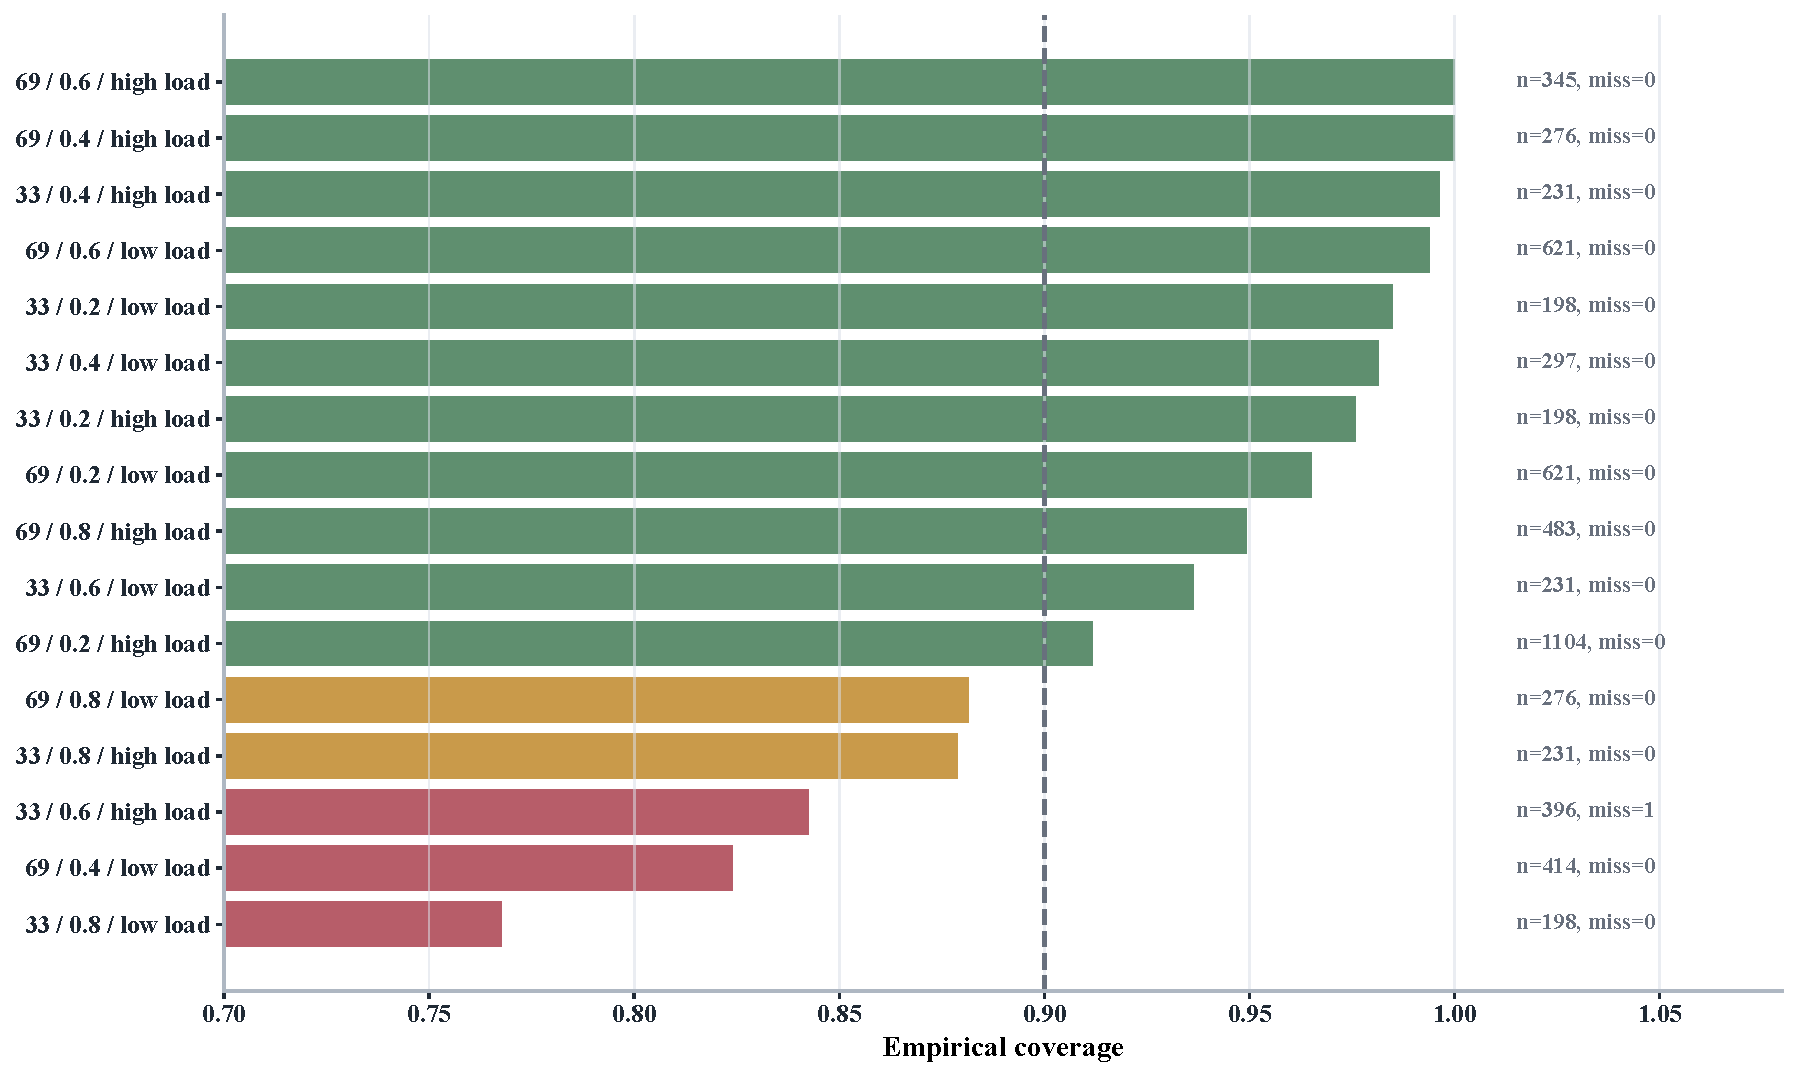
\includegraphics[width=1.1\linewidth,height=\textheight,keepaspectratio,alt={Per-family conditioned calibration audit. The bars show empirical coverage by topology/PV/loading family with sample counts and missed violations, exposing the small-family regimes where shrinkage matters.}]{figures/fig04_per_family_calibration.pdf}
\caption{Per-family conditioned calibration audit. The bars show
empirical coverage by topology/PV/loading family with sample counts and
missed violations, exposing the small-family regimes where shrinkage
matters.}\label{fig:fig04_per_family_calibration}
\end{figure}

\subsection{Risk-Stratified Calibration and
Screening}\label{risk-stratified-calibration-and-screening}

Aggregate coverage can hide the voltage-boundary behavior that matters
for operation. We therefore add a risk-stratified audit on the
representative random split. Bus samples and scenarios are grouped into
true violations, boundary-safe cases within 0.002 p.u. of either voltage
limit, near-safe cases within 0.010 p.u., and interior-safe cases. This
audit is derived from saved raw interval predictions and does not
retrain any estimator.

{\def\LTcaptype{none} % do not increment counter
\begin{longtable}[]{@{}
  >{\raggedright\arraybackslash}p{(\linewidth - 14\tabcolsep) * \real{0.1000}}
  >{\raggedright\arraybackslash}p{(\linewidth - 14\tabcolsep) * \real{0.1000}}
  >{\raggedleft\arraybackslash}p{(\linewidth - 14\tabcolsep) * \real{0.1333}}
  >{\raggedleft\arraybackslash}p{(\linewidth - 14\tabcolsep) * \real{0.1333}}
  >{\raggedleft\arraybackslash}p{(\linewidth - 14\tabcolsep) * \real{0.1333}}
  >{\raggedleft\arraybackslash}p{(\linewidth - 14\tabcolsep) * \real{0.1333}}
  >{\raggedleft\arraybackslash}p{(\linewidth - 14\tabcolsep) * \real{0.1333}}
  >{\raggedleft\arraybackslash}p{(\linewidth - 14\tabcolsep) * \real{0.1333}}@{}}
\toprule\noalign{}
\begin{minipage}[b]{\linewidth}\raggedright
Method
\end{minipage} & \begin{minipage}[b]{\linewidth}\raggedright
Stratum
\end{minipage} & \begin{minipage}[b]{\linewidth}\raggedleft
Bus samples
\end{minipage} & \begin{minipage}[b]{\linewidth}\raggedleft
Coverage
\end{minipage} & \begin{minipage}[b]{\linewidth}\raggedleft
Width
\end{minipage} & \begin{minipage}[b]{\linewidth}\raggedleft
Risk-flag rate
\end{minipage} & \begin{minipage}[b]{\linewidth}\raggedleft
Recall / false-alarm
\end{minipage} & \begin{minipage}[b]{\linewidth}\raggedleft
Missed / false alarms
\end{minipage} \\
\midrule\noalign{}
\endhead
\bottomrule\noalign{}
\endlastfoot
Boosting + global conformal & violating & 921 & 0.59501 & 0.00110 &
0.99674 & 0.99674 recall & 3 missed \\
VoltGuard & violating & 921 & 0.87188 & 0.00052 & 0.99891 & 0.99891
recall & 1 missed \\
Neural graph ablation & violating & 921 & 0.74159 & 0.00611 & 0.99783 &
0.99783 recall & 2 missed \\
Boosting + global conformal & boundary-safe & 55 & 0.78182 & 0.00110 &
0.23636 & 0.23636 false alarm & 13 false alarms \\
VoltGuard & boundary-safe & 55 & 0.92727 & 0.00044 & 0.05455 & 0.05455
false alarm & 3 false alarms \\
Neural graph ablation & boundary-safe & 55 & 0.90909 & 0.00664 & 0.81818
& 0.81818 false alarm & 45 false alarms \\
\end{longtable}
}

The boundary-safe rows are important for operating value. A conservative
interval can achieve high recall by flagging many near-limit but safe
buses, which increases unnecessary downstream AC calls or corrective
actions. VoltGuard reduces boundary-safe false-alarm buses from 13 under
boosting plus global conformal and 45 under the neural graph ablation to
three, while still missing only one of 921 truly violating buses. At
scenario level, VoltGuard recalls all 93 truly risky scenarios and
produces zero false-alarm scenarios across the boundary-safe, near-safe,
and interior-safe strata. This is a more direct voltage-risk-screening
test than aggregate RMSE alone.

\subsection{Shift and Scenario-Level
Results}\label{shift-and-scenario-level-results}

Under PV-penetration shift, VoltGuard keeps bus-level violation recall
at 99.81\%, but empirical coverage drops below nominal because the test
distribution is intentionally shifted. This is exactly why the paper
does not claim unconditional distribution-free safety. Under
topology-held-out transfer from 33-bus training to 69-bus
calibration/testing, the topology+PV+loading variant has zero missed
bus-level violations across the three seeds and lower false alarms than
boosting plus global conformal. This is encouraging, but it is still a
controlled 33-to-69 transfer with calibration on the target feeder, not
a proof of arbitrary topology-shift safety.

We also audit an explicit PV-shift recalibration protocol. The point
estimator is still trained only on the low/medium-PV split. A small,
disjoint subset of early high-PV scenarios is then treated as target
calibration, and the remaining high-PV scenarios are evaluated. This
simulates periodic AC-audited recalibration after a feeder enters a
higher renewable-hosting regime; the target calibration labels are not
reused for testing.

{\def\LTcaptype{none} % do not increment counter
\begin{longtable}[]{@{}
  >{\raggedright\arraybackslash}p{(\linewidth - 14\tabcolsep) * \real{0.0968}}
  >{\raggedleft\arraybackslash}p{(\linewidth - 14\tabcolsep) * \real{0.1290}}
  >{\raggedleft\arraybackslash}p{(\linewidth - 14\tabcolsep) * \real{0.1290}}
  >{\raggedleft\arraybackslash}p{(\linewidth - 14\tabcolsep) * \real{0.1290}}
  >{\raggedleft\arraybackslash}p{(\linewidth - 14\tabcolsep) * \real{0.1290}}
  >{\raggedleft\arraybackslash}p{(\linewidth - 14\tabcolsep) * \real{0.1290}}
  >{\raggedleft\arraybackslash}p{(\linewidth - 14\tabcolsep) * \real{0.1290}}
  >{\raggedleft\arraybackslash}p{(\linewidth - 14\tabcolsep) * \real{0.1290}}@{}}
\toprule\noalign{}
\begin{minipage}[b]{\linewidth}\raggedright
PV-shift calibration protocol
\end{minipage} & \begin{minipage}[b]{\linewidth}\raggedleft
Target high-PV calibration scenarios
\end{minipage} & \begin{minipage}[b]{\linewidth}\raggedleft
High-PV test scenarios
\end{minipage} & \begin{minipage}[b]{\linewidth}\raggedleft
Coverage
\end{minipage} & \begin{minipage}[b]{\linewidth}\raggedleft
Width
\end{minipage} & \begin{minipage}[b]{\linewidth}\raggedleft
Recall
\end{minipage} & \begin{minipage}[b]{\linewidth}\raggedleft
False alarm
\end{minipage} & \begin{minipage}[b]{\linewidth}\raggedleft
Missed
\end{minipage} \\
\midrule\noalign{}
\endhead
\bottomrule\noalign{}
\endlastfoot
Source PV 0.6 calibration only & 0 & 132 & 0.76915 & 0.00081 & 0.99807 &
0.00147 & 1.00 \\
Source + 10\% target high-PV calibration & 16 & 116 & 0.89527 & 0.00189
& 1.00000 & 0.00398 & 0.00 \\
Source + 20\% target high-PV calibration & 29 & 103 & 0.88790 & 0.00176
& 1.00000 & 0.00322 & 0.00 \\
\end{longtable}
}

Thus target recalibration repairs much of the coverage loss and removes
the remaining missed bus-level violation, but it does so by widening
intervals and raising false alarms. This is not an unconditional
conformal guarantee under PV shift; it is evidence that the screening
layer can be re-calibrated when a new high-PV operating regime supplies
AC-audited calibration cases.

The same PV-shift adaptation is also translated into operating screening
quantities on the remaining high-PV scenarios. With source-only
calibration, VoltGuard releases 57.00 high-PV scenarios from downstream
AC optimization on average, but still has one missed bus-level
violation. Adding the 10\% target high-PV calibration set removes the
bus-level missed violation while keeping scenario-level risky recall at
1.00000. The cost is operationally visible: screened-safe releases fall
to 49.67 scenarios and the mean interval width increases from 0.00081 to
0.00209 p.u. This is the desired interpretation for energy management:
target recalibration improves high-PV risk conservatism, but it consumes
calibration data and reduces the number of scenarios that can be safely
bypassed.

{\def\LTcaptype{none} % do not increment counter
\begin{longtable}[]{@{}
  >{\raggedright\arraybackslash}p{(\linewidth - 12\tabcolsep) * \real{0.1111}}
  >{\raggedleft\arraybackslash}p{(\linewidth - 12\tabcolsep) * \real{0.1481}}
  >{\raggedleft\arraybackslash}p{(\linewidth - 12\tabcolsep) * \real{0.1481}}
  >{\raggedleft\arraybackslash}p{(\linewidth - 12\tabcolsep) * \real{0.1481}}
  >{\raggedleft\arraybackslash}p{(\linewidth - 12\tabcolsep) * \real{0.1481}}
  >{\raggedleft\arraybackslash}p{(\linewidth - 12\tabcolsep) * \real{0.1481}}
  >{\raggedleft\arraybackslash}p{(\linewidth - 12\tabcolsep) * \real{0.1481}}@{}}
\toprule\noalign{}
\begin{minipage}[b]{\linewidth}\raggedright
PV-shift screening protocol
\end{minipage} & \begin{minipage}[b]{\linewidth}\raggedleft
Target high-PV calibration scenarios
\end{minipage} & \begin{minipage}[b]{\linewidth}\raggedleft
AC calls avoided mean
\end{minipage} & \begin{minipage}[b]{\linewidth}\raggedleft
Risky recall mean
\end{minipage} & \begin{minipage}[b]{\linewidth}\raggedleft
Post-screen miss mean
\end{minipage} & \begin{minipage}[b]{\linewidth}\raggedleft
Missed buses mean
\end{minipage} & \begin{minipage}[b]{\linewidth}\raggedleft
Width mean
\end{minipage} \\
\midrule\noalign{}
\endhead
\bottomrule\noalign{}
\endlastfoot
Source PV 0.6 calibration only & 0 & 57.00 & 1.00000 & 0.00000 & 1.00 &
0.00081 \\
Source + 10\% target high-PV calibration & 16 & 49.67 & 1.00000 &
0.00000 & 0.00 & 0.00209 \\
\end{longtable}
}

At scenario level, the representative random split has 120 test
scenarios and 93 risky scenarios. VoltGuard topology+PV+loading
conditioned calibration has scenario recall 1.000, zero missed risky
scenarios, and zero scenario false alarms. The neural graph ablation
also avoids missed risky scenarios but triggers many more scenario false
alarms and has worse bus-level sharpness.

\begin{figure}
\centering
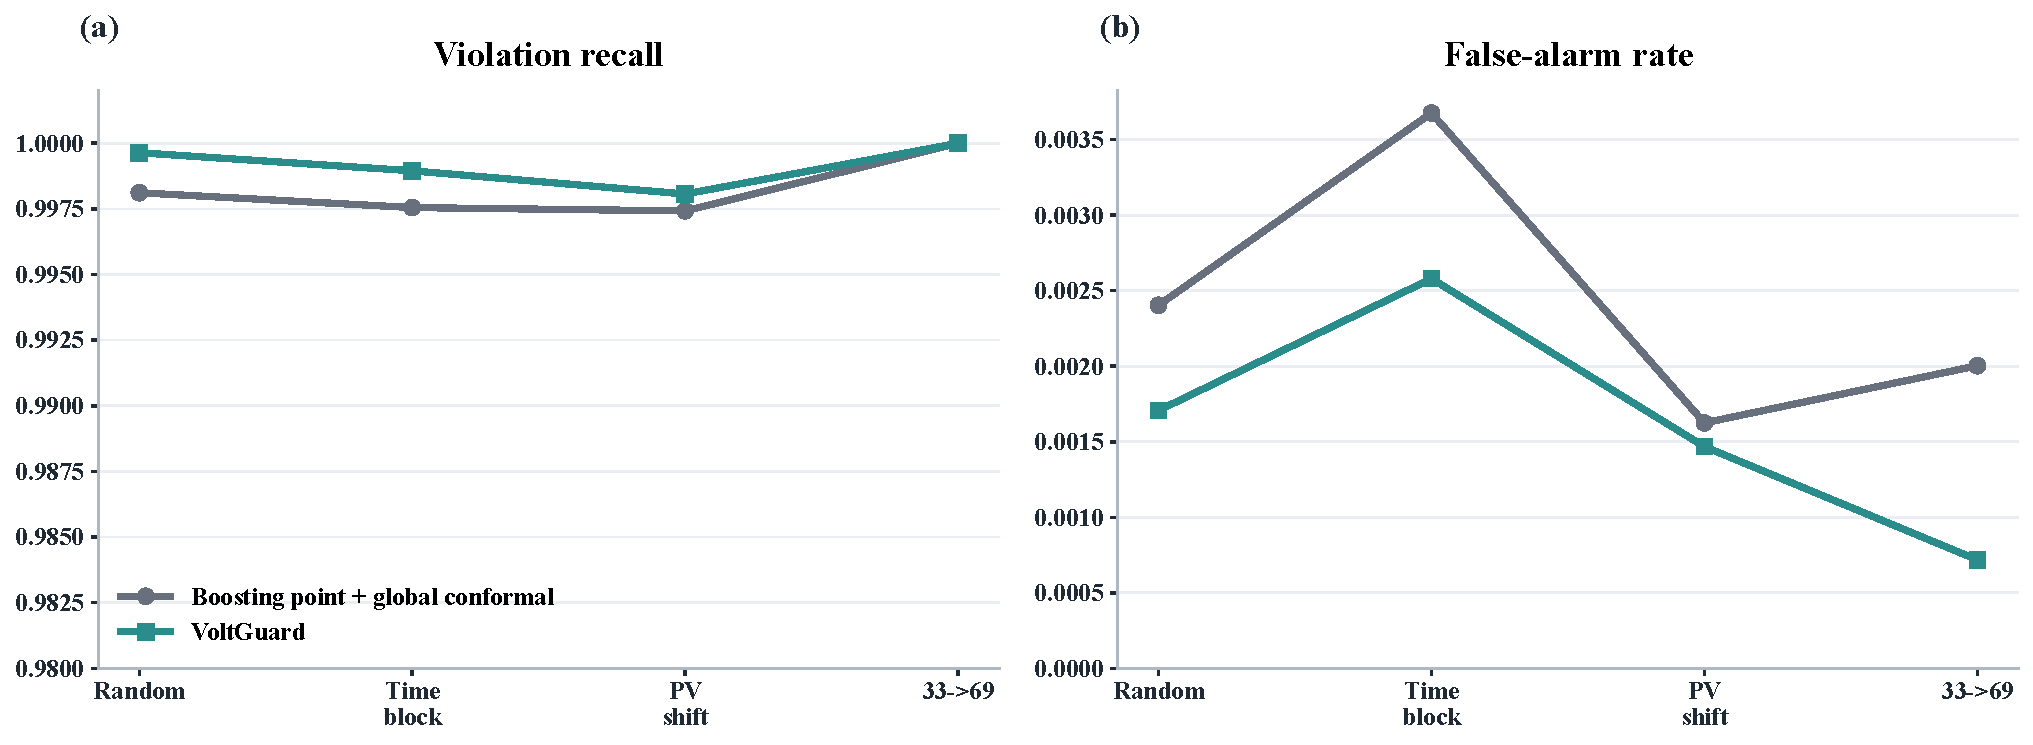
\includegraphics[width=1.1\linewidth,height=\textheight,keepaspectratio,alt={Shift generalization across time, PV penetration, and topology transfer. (a) Multi-seed violation recall under random, synthetic time-block, PV-shift, and topology-transfer splits; (b) corresponding false-alarm rates.}]{figures/fig05_shift_generalization.pdf}
\caption{Shift generalization across time, PV penetration, and topology
transfer. (a) Multi-seed violation recall under random, synthetic
time-block, PV-shift, and topology-transfer splits; (b) corresponding
false-alarm rates.}\label{fig:fig05_shift_generalization}
\end{figure}

\subsection{Expanded IEEE 118-Bus Stress
Audit}\label{expanded-ieee-118-bus-stress-audit}

The IEEE 118-bus case is not used as the main distribution-network
evidence, but the review requested either a realistic feeder case or a
more complete analysis of this supplementary system. We therefore report
the same representative random-split metrics on the 118-bus stress case.
The result is intentionally interpreted as a stress audit because the
LinDistFlow assumptions and radial distribution-feeder interpretation
are not native to this system.

{\def\LTcaptype{none} % do not increment counter
\begin{longtable}[]{@{}
  >{\raggedright\arraybackslash}p{(\linewidth - 14\tabcolsep) * \real{0.1000}}
  >{\raggedright\arraybackslash}p{(\linewidth - 14\tabcolsep) * \real{0.1000}}
  >{\raggedleft\arraybackslash}p{(\linewidth - 14\tabcolsep) * \real{0.1333}}
  >{\raggedleft\arraybackslash}p{(\linewidth - 14\tabcolsep) * \real{0.1333}}
  >{\raggedleft\arraybackslash}p{(\linewidth - 14\tabcolsep) * \real{0.1333}}
  >{\raggedleft\arraybackslash}p{(\linewidth - 14\tabcolsep) * \real{0.1333}}
  >{\raggedleft\arraybackslash}p{(\linewidth - 14\tabcolsep) * \real{0.1333}}
  >{\raggedleft\arraybackslash}p{(\linewidth - 14\tabcolsep) * \real{0.1333}}@{}}
\toprule\noalign{}
\begin{minipage}[b]{\linewidth}\raggedright
Method
\end{minipage} & \begin{minipage}[b]{\linewidth}\raggedright
Variant
\end{minipage} & \begin{minipage}[b]{\linewidth}\raggedleft
RMSE
\end{minipage} & \begin{minipage}[b]{\linewidth}\raggedleft
Coverage
\end{minipage} & \begin{minipage}[b]{\linewidth}\raggedleft
Width
\end{minipage} & \begin{minipage}[b]{\linewidth}\raggedleft
Recall
\end{minipage} & \begin{minipage}[b]{\linewidth}\raggedleft
False alarm
\end{minipage} & \begin{minipage}[b]{\linewidth}\raggedleft
Missed
\end{minipage} \\
\midrule\noalign{}
\endhead
\bottomrule\noalign{}
\endlastfoot
LinDistFlow physical backbone & none & 0.88711 & n/a & n/a & 0.80723 &
0.87352 & 48 \\
Random forest & none & 0.00445 & n/a & n/a & 0.58635 & 0.00425 & 103 \\
Gradient boosting & none & 0.00466 & n/a & n/a & 0.57831 & 0.00586 &
105 \\
Boosting point + global conformal & global & 0.00466 & 0.89237 & 0.01005
& 0.82731 & 0.06236 & 43 \\
VoltGuard topology-aware residual & global & 0.00572 & 0.90254 & 0.01054
& 0.81526 & 0.06851 & 46 \\
VoltGuard topology-aware residual & PV conditioned & 0.00572 & 0.91243 &
0.01211 & 0.88755 & 0.07159 & 28 \\
VoltGuard topology-aware residual & topology/PV/loading & 0.00572 &
0.91328 & 0.01211 & 0.88353 & 0.07100 & 29 \\
\end{longtable}
}

The 118-bus audit does not strengthen the distribution-feeder claim; it
exposes where the present physical backbone is inappropriate. The stress
case requires much wider intervals and still misses more bus-level
violations than the 33/69 distribution-feeder experiments. This is why
the main evidence is kept on IEEE 33-bus and 69-bus feeders, while
realistic unbalanced OpenDSS/SMART-DS feeders remain a required next
validation step rather than a claim made by the current manuscript.

\subsection{Failure Mode Analysis}\label{failure-mode-analysis}

The representative 33/69 random split contains one missed bus-level
violation for the selected topology/PV/loading conditioned VoltGuard
interval. The miss occurs on IEEE 33-bus scenario 153, bus 7, under PV
bin 0.6 and high loading. The true voltage is 0.949940 p.u., only
0.000060 p.u. below the 0.95 p.u. limit. The predicted voltage is
0.950518 p.u.; with a conformal radius of 0.000351 p.u., the lower
interval endpoint is 0.950167 p.u. and therefore just misses the
undervoltage boundary.

This is not a missed risky scenario. The same scenario contains many
deeper undervoltage buses, including bus 17 at 0.916314 p.u. and bus 16
at 0.917032 p.u., all of which are flagged by the interval screen. The
failure mode is therefore a boundary-bus miss inside an already risky
scenario, not a release of a dangerous scenario. Operationally, the
scenario would still enter the corrective-audit queue because other
buses are flagged.

The early-warning indicators are visible in the inputs: high loading, PV
bin 0.6, multiple downstream buses near the undervoltage band, and a
scenario whose minimum interval lower bound is already far below 0.95
p.u. The DMS integration paper turns these indicators into fallback
rules: stale telemetry, unseen topology, out-of-envelope forecast
features, and rolling residual alarms force watch or corrective-audit
routing even when an individual boundary bus is not flagged.

\subsection{Computational Cost and Breakeven
Analysis}\label{computational-cost-and-breakeven-analysis}

The reviewer-requested timing audit separates training, online
screening, and downstream AC-audited grid search. On the representative
random split, fitting the residual learner uses 18,360 training rows and
takes 1.858 s; the full train/calibration/test evaluation takes 4.468 s.
The supplementary 118-bus stress run takes 2.426 s for model fitting and
2.508 s end-to-end.

{\def\LTcaptype{none} % do not increment counter
\begin{longtable}[]{@{}
  >{\raggedright\arraybackslash}p{(\linewidth - 8\tabcolsep) * \real{0.1579}}
  >{\raggedleft\arraybackslash}p{(\linewidth - 8\tabcolsep) * \real{0.2105}}
  >{\raggedleft\arraybackslash}p{(\linewidth - 8\tabcolsep) * \real{0.2105}}
  >{\raggedleft\arraybackslash}p{(\linewidth - 8\tabcolsep) * \real{0.2105}}
  >{\raggedleft\arraybackslash}p{(\linewidth - 8\tabcolsep) * \real{0.2105}}@{}}
\toprule\noalign{}
\begin{minipage}[b]{\linewidth}\raggedright
Workflow
\end{minipage} & \begin{minipage}[b]{\linewidth}\raggedleft
Scenarios sent to AC
\end{minipage} & \begin{minipage}[b]{\linewidth}\raggedleft
Seconds
\end{minipage} & \begin{minipage}[b]{\linewidth}\raggedleft
ms/scenario
\end{minipage} & \begin{minipage}[b]{\linewidth}\raggedleft
Speedup vs full AC
\end{minipage} \\
\midrule\noalign{}
\endhead
\bottomrule\noalign{}
\endlastfoot
VoltGuard online screening only & 120 & 0.03046 & 0.25380 & 6796.17 \\
Full AC grid search on every scenario & 120 & 206.98291 & 1724.86 &
1.00 \\
VoltGuard-flagged scenarios then AC grid search & 93 & 160.44221 &
1725.19 & 1.29 \\
VoltGuard top-20\% budget then AC grid search & 24 & 41.42704 & 1726.13
& 5.00 \\
\end{longtable}
}

A rough breakeven calculation is favorable because online screening is
cheap. Using the 1.858 s fit time and the per-scenario difference
between full AC grid search and screening-only evaluation, the fit cost
is recovered after roughly 1.1 screened scenarios. The more important
operational question is not training amortization but triage policy:
conservative intervals may still send many scenarios to AC analysis,
while risk-budgeted queues can reduce wall-clock time when the operator
has a limited AC-study budget.

\section{Discussion}\label{discussion}

The central result is a corrected claim, not a broader one. The best
executed model is not a neural graph residual. It is a physics-informed,
topology-aware residual learner with conditioned conformal calibration.
This makes the paper more defensible: the method's value comes from
aligning the residual features and calibration families with feeder and
operating regime, not from claiming that message passing alone solves
voltage security.

The conformal guarantee is bounded. Split conformal prediction provides
finite-sample coverage under exchangeability of calibration and test
samples. Grid data can violate this assumption when topology, load
regimes, PV penetration, or time periods shift. The PV-shift and
topology-held-out experiments make that limitation visible rather than
hiding it. VoltGuard should therefore be used as a calibrated screening
estimator under a stated scenario family and recalibration protocol, not
as a universal safety certificate.

The screening interpretation is also bounded. The intervals can
prioritize scenarios and buses for downstream AC analysis, but they do
not certify AC feasibility, replace state estimation, or select final
dispatch. OPF, MPC, and AC power flow remain the authority for
corrective action. This distinction is important for reviewer
interpretation: the paper's claim is sharper intervals and fewer missed
voltage-risk events than baseline screening methods, not a new
distribution-grid controller.

Model maintenance is part of the operating design. A deployed screen
should store every model version, feeder model, calibration family, and
release/watch decision, then sample released scenarios for periodic AC
audit. Recalibration should be triggered when rolling residuals exceed
the calibration-family threshold, when topology identifiers are unseen,
when DER capacity or siting changes materially, when
reconductoring/regulator/capacitor settings change, or when forecast
distributions move outside the training envelope. In those cases the DMS
should disable release or fall back to a global conservative radius
until a fresh AC-audited calibration set is available.

Real-world validation remains the most important external gap. The
present evidence uses public IEEE-style test systems and synthetic
operating scenarios; it does not include an anonymized utility feeder,
real SCADA/AMI streams, or an OpenDSS/SMART-DS unbalanced feeder with
regulator, capacitor, and phase connectivity details. On real feeders,
missing telemetry, phase imbalance, equipment controls, and
data-governance rules may dominate the residual structure. The current
results should therefore be read as a reproducible method demonstration
and screening benchmark, while utility-pilot validation is required
before operational deployment claims.

The present feeder models are balanced single-phase equivalents, so
extension to highly unbalanced three-phase distribution systems is not
automatic. On IEEE 123-bus or OpenDSS feeders, the LinDistFlow backbone
would need a phase-resolved branch-flow approximation with
phase-specific voltage limits, mutual coupling terms, regulator and
capacitor states, and missing-phase connectivity. The residual learner
can still use the same philosophy, but its features would become
phase-indexed and equipment-aware, and the conformal families would
likely need to include regulator configuration, phase loading, and
feeder section. This is a limitation of the current 33/69 evidence.

\section{Conclusion}\label{conclusion}

This paper presents VoltGuard, a physics-informed topology-aware
residual learning framework with conformal calibration for voltage-risk
screening in active distribution networks. On IEEE 33-bus and IEEE
69-bus feeder scenarios, the topology+PV+loading conditioned conformal
variant improves missed-violation and interval-sharpness behavior
relative to global conformal calibration. The work deliberately keeps
neural graph residual learning as an ablation because the executed
neural model does not justify being the central claim. Future work will
extend the same residual-plus-conditioned-calibration framework to
unbalanced IEEE 123-bus/OpenDSS or SMART-DS feeders and evaluate
recalibration under larger topology and DER regime shifts.

\section*{Declaration of Competing
Interest}\label{declaration-of-competing-interest}
\addcontentsline{toc}{section}{Declaration of Competing Interest}

The authors declare that they have no known competing financial
interests or personal relationships that could have appeared to
influence the work reported in this paper.

\section*{Funding}\label{funding}
\addcontentsline{toc}{section}{Funding}

This research did not receive any specific grant from funding agencies
in the public, commercial, or not-for-profit sectors.

\section*{Code and Data Availability}\label{code-and-data-availability}
\addcontentsline{toc}{section}{Code and Data Availability}

The experiments use publicly available IEEE test systems implemented
through pandapower and a project-local IEEE 69-bus feeder
implementation. The local reproducibility package includes the scenario
generator, configured evaluation pipeline, conformal calibration code,
raw predictions, conformal scores, runtime tables, post-action AC audit
outputs, DMS prototype logs, reviewer-requested baseline comparisons,
and energy-management value metrics. File-level checksums and
reproduction commands are recorded in
\texttt{experiments/results/reproducibility\_manifest.json} and
\texttt{experiments/results/reproducibility\_manifest.md}. The Python
implementation, synthetic scenario-generation scripts, trained model
artifacts, table-generation scripts, manuscript sources, and release
PDFs are publicly archived at
\texttt{https://github.com/Zhaosiqiang/voltguard-voltage-risk-screening/releases/tag/v1.0.0-submission}.
A Zenodo DOI will be added after the GitHub repository is connected to
Zenodo by the account owner.

\section*{Declaration of Generative AI and AI-Assisted Technologies in
the Writing
Process}\label{declaration-of-generative-ai-and-ai-assisted-technologies-in-the-writing-process}
\addcontentsline{toc}{section}{Declaration of Generative AI and
AI-Assisted Technologies in the Writing Process}

During the preparation of this work, the authors used AI-assisted coding
and language tools for drafting support, code scaffolding, consistency
checks, and language refinement. The authors reviewed and edited all
generated text and code, verified the equations and numerical claims,
and take full responsibility for the content of the article.

\section*{References}\label{references}
\addcontentsline{toc}{section}{References}

{[}1{]} Baran ME, Wu FF. Network reconfiguration in distribution systems
for loss reduction and load balancing. IEEE Transactions on Power
Delivery. 1989;4(2):1401-1407. https://doi.org/10.1109/61.25627.

{[}2{]} Dall'Anese E, Zhu H, Giannakis GB. Optimal power flow for
distribution networks under constraints. IEEE Transactions on Smart
Grid. 2013;4(3):1460-1471. https://doi.org/10.1109/TSG.2013.2247644.

{[}3{]} Molzahn DK, Dorfler F, Sandberg H, Low SH, Chakrabarti S,
Baldick R, et al.~A survey of distributed optimization and control
algorithms for electric power systems. IEEE Transactions on Smart Grid.
2017;8(6):2941-2962. https://doi.org/10.1109/TSG.2017.2720471.

{[}4{]} Bertrand A, Donnot B, Marot A, Guyon I. Physics-informed
graphical neural network for power system state estimation. Applied
Energy. 2024;358:122602.

{[}5{]} Kipf TN, Welling M. Semi-supervised classification with graph
convolutional networks. International Conference on Learning
Representations. 2017.

{[}6{]} Hamilton WL, Ying Z, Leskovec J. Inductive representation
learning on large graphs. Advances in Neural Information Processing
Systems. 2017;30.

{[}7{]} Vovk V, Gammerman A, Shafer G. Algorithmic Learning in a Random
World. Springer; 2005. https://doi.org/10.1007/b106715.

{[}8{]} Shafer G, Vovk V. A tutorial on conformal prediction. Journal of
Machine Learning Research. 2008;9:371-421.

{[}9{]} Romano Y, Patterson E, Candes E. Conformalized quantile
regression. Advances in Neural Information Processing Systems. 2019;32.

{[}10{]} Zargarbashi SH, Antonelli S, Bojchevski A. Conformal prediction
sets for graph neural networks. Proceedings of the 40th International
Conference on Machine Learning. PMLR. 2023;202:12292-12318.

{[}11{]} Huang K, Jin Y, Candes E, Leskovec J. Uncertainty
quantification over graph with conformalized graph neural networks.
Advances in Neural Information Processing Systems. 2023;36.

{[}12{]} Farivar M, Low SH. Branch flow model: relaxations and
convexification, Part I. IEEE Transactions on Power Systems.
2013;28(3):2554-2564. https://doi.org/10.1109/TPWRS.2013.2255317.

{[}13{]} Gan L, Low SH. Convex relaxations and linear approximation for
optimal power flow in multiphase radial networks. Power Systems
Computation Conference. 2014.

{[}14{]} Bernstein A, Dall'Anese E, Simonetto A. Online primal-dual
methods with measurement feedback for time-varying convex optimization.
IEEE Transactions on Signal Processing. 2019;67(8):1978-1991.

{[}15{]} Turitsyn K, Sulc P, Backhaus S, Chertkov M. Options for control
of reactive power by distributed photovoltaic generators. Proceedings of
the IEEE. 2011;99(6):1063-1073.

{[}16{]} Robbins BA, Hadjicostis CN, Dominguez-Garcia AD. A two-stage
distributed architecture for voltage control in power distribution
systems. IEEE Transactions on Power Systems. 2013;28(2):1470-1482.

{[}17{]} Zamzam AS, Baker K. Learning optimal solutions for extremely
fast AC optimal power flow. IEEE Power \& Energy Society General
Meeting. 2019.

{[}18{]} Donti PL, Rolnick D, Kolter JZ. DC3: a learning method for
optimization with hard constraints. International Conference on Learning
Representations. 2021.

{[}19{]} Zamzam AS, Sidiropoulos ND. Physics-aware neural networks for
distribution system state estimation. IEEE Transactions on Power
Systems. 2020;35(6):4347-4356.

{[}20{]} Karagiannopoulos S, Aristidou P, Hug G. Data-driven local
control design for active distribution grids using off-line optimal
power flow and machine learning techniques. IEEE Transactions on Smart
Grid. 2019;10(6):6461-6471.

{[}21{]} Sankur MD, Dobbe R, Stewart E, Arnold D, Callaway D. A
linearized power flow model for optimization in unbalanced distribution
systems. IEEE Transactions on Power Systems. 2016;31(4):2755-2763.

{[}22{]} Kivaranovic D, Johnson KD, Leeb H. Adaptive, distribution-free
prediction intervals for deep networks. Proceedings of the 23rd
International Conference on Artificial Intelligence and Statistics.
PMLR. 2020;108:4346-4356.

{[}23{]} Angelopoulos AN, Bates S. A gentle introduction to conformal
prediction and distribution-free uncertainty quantification. Foundations
and Trends in Machine Learning. 2023;16(4):494-591.

{[}24{]} Barber RF, Candes EJ, Ramdas A, Tibshirani RJ. Predictive
inference with the jackknife+ and cross-validation+. Annals of
Statistics. 2021;49(1):486-507.

{[}25{]} IEEE PES Distribution System Analysis Subcommittee. IEEE PES
distribution test feeders. IEEE Power \& Energy Society; accessed 2026.

{[}26{]} Palmintier B, Elgindy T, Mateo C, Giraldez J, Hodge BM.
SMART-DS: synthetic models for advanced, realistic testing: distribution
systems and scenarios. National Renewable Energy Laboratory. 2020.

{[}27{]} International Electrotechnical Commission. IEC 61970: Energy
management system application program interface (EMS-API): Common
Information Model. IEC; current edition.

{[}28{]} International Electrotechnical Commission. IEC 61968:
Application integration at electric utilities: System interfaces for
distribution management. IEC; current edition.

{[}29{]} IEEE Standards Association. IEEE Std 2030.5: Smart Energy
Profile Application Protocol. IEEE; current edition.

{[}30{]} Open Field Message Bus Consortium. OpenFMB framework and data
model specification. OpenFMB; current edition.

\end{document}
